%================================================================
% SLO
%----------------------------------------------------------------
% datoteka: 	thesis_template.tex
%
% opis: 		predloga za pisanje diplomskega dela v formatu LaTeX na
% 				Univerza v Ljubljani, Fakulteti za računalništvo in informatiko
%
% pripravili: 	Matej Kristan, Zoran Bosnić, Andrej Čopar,
%			  	po začetni predlogi Gašperja Fijavža
%
% popravil: 	Domen Rački, Jaka Cikač, Matej Kristan
%
% verzija: 		30. september 2016 (dodan razširjeni povzetek)
%================================================================


%================================================================
% SLO: definiraj strukturo dokumenta
% ENG: define file structure
%================================================================
\documentclass[a4paper, 12pt]{book}
\usepackage{makecell}
%================================================================
% SLO: Odkomentiraj "\SLOtrue " za izbiro slovenskega jezika
% ENG: Uncomment "\SLOfalse" to chose English languagge
%================================================================
\newif\ifSLO
\newif\ifTRACKEXIST
\newif\ifTRACKCS
\newif\ifPROGRAMMM
\newif\ifPROGRAMEMAI


% ---------------------------------------------------------------------------------------
% IMPORTANT: Adjust the thesis language, your study program and track within this block
% ---------------------------------------------------------------------------------------
% ** switch language ** %
%\SLOtrue % Enables Slovenian language
\SLOfalse  % Enables English language

% ** Switch programs: ** %

% ** Uncomment if Program: Computer Science, Track: Computer Science **%
\TRACKCStrue
\TRACKEXISTtrue

% ** Uncomment if Program: Computer Science, Track: Data Science **%
%\TRACKCSfalse
%\TRACKEXISTtrue

% ** Uncomment if Program: Multimedia **%
%\PROGRAMMMtrue 
%\TRACKEXISTfalse 

% ** Uncomment if Program: EMAI **%
%\PROGRAMEMAItrue
%\SLOfalse 

% -------------------------------------------------------------------------------------------
% End of language, program and track adjustment
% -------------------------------------------------------------------------------------------


%================================================================
% SLO: vključi oblikovanje in pakete
% ENG: include design and packages
%================================================================
%----------------------------------------------------------------
% SLO: LaTeX paketi
% ENG: LateX packages
%----------------------------------------------------------------
% SLO: omogoča uporabo slovenskih (latinskih) črk kodiranih v formatu UTF-8
% ENG: enables the use of slovene (latin) caracters encoded in the UFT-8 format
\usepackage[utf8x]{inputenc}
%\inputencoding{utf8}
% SLO: naloži, med drugim, slovenske delilne vzorce
% ENG: loads, among others, slovene dividing patterns
\usepackage[slovene,english]{babel}
% SLO: poskrbi za postavitev strani
% ENG: takes care of the page layout
\usepackage{fancyhdr}
% SLO: za vlaganje slik različnih formatov
% ENG: for loading figures of different formats
\usepackage{graphicx}
\usepackage{caption}
\usepackage{multirow}
\usepackage{todonotes}
\captionsetup[figure]{labelfont=bf} % SLO: napis "Slika #" v krepkem tisku
									% ENG: wirte "Figure #" caption in bold
\captionsetup[table]{labelfont=bf} % SLO: napis "Tabela #" v krepkem tisku
								   % ENG: wirte "Table #" caption in bold
% SLO: za pisanje psevdokode
% ENG: for writing pseudocode
\usepackage{algorithm}
\usepackage{algorithmic}
\floatname{algorithm}{\footnotesize Algorithm} % SLO: napis "Algoritem #" v krepkem tisku
											   % ENG: write "Algorithm #" caption in bold
% SLO: poveže reference slik/tabel in slike/tabele znotraj dokumenta
% ENG: links image/table references with the images/tables within the document
\usepackage[pdfa]{hyperref}
% SLO: pri kliku na referenco slike/tabele se postavi na vrh slike/tabele
% ENG: when clicking the image/table reference, position the focus on top of the image/table
\usepackage[all]{hypcap}
% SLO: omogoča, med drugim, definicjo in uporebo barve
% ENG: enables, among others, the definition and use of colors
\usepackage{xcolor}
%----------------------------------------------------------------
% SLO: dodatni paketi
% ENG: additional packages
%----------------------------------------------------------------
% SLO: omogoča večjo manipulacijo nad tabelami
% ENG: allows for greater manipulation of tables
\usepackage{booktabs}
% SLO: naloži dodatne simbole
% ENG: loads additional symbols
\usepackage{amssymb}
% SLO: omogoča, med drugim, sklicevanje na formule z eqref
% ENG: enables, among others, equation referencing with eqref
\usepackage{amsmath}
% SLO: omogoča komentiranje večjega dela teksta
% ENG: enables the commenting of larger text parts
\usepackage{verbatim}
% SLO: omogoča rotacijo PDF strani v ležeč položaj
% ENG: enables the rotation of a PDF page to landscape
\usepackage{pdflscape}
% SLO: omogoča barvanje vrstic in stolpcev tabel
% ENG: enables coloring of table rows and columns
\usepackage{colortbl}
\usepackage{url}



%================================================================
% SLO: nastavitve dokumenta
% ENG: document properties
%================================================================
% SLO: prilagoditev robov za tisk
% ENG: margin adjustments for printing
\addtolength{\marginparwidth}{-20pt}
\addtolength{\oddsidemargin}{40pt}
\addtolength{\evensidemargin}{-40pt}
% SLO: razmik med vrsticami
% ENG: line spacing
\renewcommand{\baselinestretch}{1.3}
% SLO: postavitev strani
% ENG: page layout
\renewcommand{\chaptermark}[1]{\markboth{\MakeUppercase{\thechapter.\ #1}}{}}
\renewcommand{\sectionmark}[1]{\markright{\MakeUppercase{\thesection.\ #1}}}
\renewcommand{\headrulewidth}{0.5pt} % Header rule
\renewcommand{\footrulewidth}{0pt} % Footer rule
%
\fancypagestyle{frontmatter}{%
	\fancyhf{} % Clear all headers and footers first
	\fancyhead[LE, RO]{\sl \thepage}
	%\fancyhead[LO]{\sl \rightmark}
	%\fancyhead[RE]{\sl \leftmark}
}
\fancypagestyle{mainmatter}{%
  	\fancyhf{} % Clear all headers and footers first
	\fancyhead[LE,RO]{\sl \thepage}
	\fancyhead[LO]{\sl \rightmark}
	\fancyhead[RE]{\sl \leftmark}
}
% SLO: font za ime avtorja
% ENG: font for author name
\newcommand{\authorfont}{\Large}
% SLO: font za naslov diplomskega dela
% ENG: font for thesis title
\newcommand{\titlefont}{\LARGE\bf}
% SLO: globina kazala
% ENG: content depth
\setcounter{tocdepth}{1}
% SLO: definiraj ukaz za prazno stran
% ENG: define the command for empty page
\newcommand{\clearemptydoublepage}{\newpage{\pagestyle{empty}\cleardoublepage}}

% course title
\newcommand{\trackname}{!undefined!}

\newcommand{\BibTeX}{{\sc Bib}\TeX}




%----------------------------------------------------------------
% |||||||||||||||||||||| USTREZNO POPRAVI |||||||||||||||||||||||
% |||||||||||||||||||||| EDIT ACCORDINGLY |||||||||||||||||||||||
%----------------------------------------------------------------
\newcommand{\ttitle}{Na transformerjih osnovano ogrodje za posplošljivo označevanje faz spanja na podlagi elektroencefalografskih podatkov}
\newcommand{\ttitleEn}{A Transformer-Based Framework for Generalizable Sleep Staging from Electroencephalography Data}
\newcommand{\tsubject}{\ttitle}
\newcommand{\tsubjectEn}{\ttitleEn}
\newcommand{\tauthor}{Matej Klančar}
\newcommand{\temail}{klancar.matej@gmail.com}
\newcommand{\myyear}{2026}
\newcommand{\tkeywords}{označevanje faz, transformerji, prenosno učenje, domenska posplošljivost}
\newcommand{\tkeywordsEn}{sleep staging, transformers, transfer learning, domain generalization}
\newcommand{\mysupervisor}{izr. prof. dr. Jure Demšar}
% Uncomment and define the following definition if you have a co-supervisor
%\newcommand{\mycosupervisor}{akad.~prof.~dr.\ Martin Krpan}
 

%%  Code publication under GNU
% NOTE: If you chose to publish the source code as part of the thesis, then put the url here and change the appropriate switch below !!
\newcommand{\linktosourcecode}{https://github.com/selenci/masters-sleep-stage-detection}
\newif\ifCODEPUBLISHED

% Chosing the published code "true" will automatically generate the licence statement for the code on the licence page.
 \CODEPUBLISHEDtrue % uncomment if the code is published
% \CODEPUBLISHEDfalse % uncomment if the code is not published
%% End of Code publication under GNU

% include formatted front pages

%----------------------------------------------------------------
% SLO: definiraj metapodatke za datoteko thesis_template.tex
% ENG: define metadata for the file thesis_template.tex
%----------------------------------------------------------------
%----------------------------------------------------------------
%	HYPERREF SETUP
% SLO: ustrezno popravi e-mail
% ENG: edit the e-mail accordingly
%----------------------------------------------------------------
\hypersetup{pdftitle={\ttitle}}
\hypersetup{pdfsubject=\ttitleEn}
\hypersetup{pdfauthor={\tauthor, \temail}}
\hypersetup{pdfkeywords=\tkeywordsEn}

%----------------------------------------------------------------
% define medatata
% SLO: ustrezno popravi e-mail
% ENG: edit the e-mail accordingly
%----------------------------------------------------------------
\def\Title{\ttitle}
\def\Author{\tauthor, \temail}
\def\Subject{\ttitleEn}
\def\Keywords{\tkeywordsEn}
\def\Org{Univerza v Ljubljani, Fakulteta za računalništvo in informatiko}

%%%%%%%%%%%%%%%%%%%%%%%%%%%%%%%%%%%%%%%%
% \convertDate converts D:20080419103507+02'00' to 2008-04-19T10:35:07+02:00
%%%%%%%%%%%%%%%%%%%%%%%%%%%%%%%%%%%%%%%%
\def\convertDate{%
    \getYear
}

{\catcode`\D=12
 \gdef\getYear D:#1#2#3#4{\edef\xYear{#1#2#3#4}\getMonth}
}
\def\getMonth#1#2{\edef\xMonth{#1#2}\getDay}
\def\getDay#1#2{\edef\xDay{#1#2}\getHour}
\def\getHour#1#2{\edef\xHour{#1#2}\getMin}
\def\getMin#1#2{\edef\xMin{#1#2}\getSec}
\def\getSec#1#2{\edef\xSec{#1#2}\getTZh}
\def\getTZh +#1#2{\edef\xTZh{#1#2}\getTZm}
\def\getTZm '#1#2'{%
    \edef\xTZm{#1#2}%
    \edef\convDate{\xYear-\xMonth-\xDay T\xHour:\xMin:\xSec+\xTZh:\xTZm}%
}

\expandafter\convertDate\pdfcreationdate


%%%%%%%%%%%%%%%%%%%%%%%%%%%%%%%%%%%%%%%%
% get pdftex version string
%%%%%%%%%%%%%%%%%%%%%%%%%%%%%%%%%%%%%%%%
\newcount\countA
\countA=\pdftexversion
\advance \countA by -100
\def\pdftexVersionStr{pdfTeX-1.\the\countA.\pdftexrevision}

%%%%%%%%%%%%%%%%%%%%%%%%%%%%%%%%%%%%%%%%
% XMP data
%%%%%%%%%%%%%%%%%%%%%%%%%%%%%%%%%%%%%%%%
\usepackage{xmpincl}
\includexmp{pdfa-1b}

%%%%%%%%%%%%%%%%%%%%%%%%%%%%%%%%%%%%%%%%
% pdfInfo
%%%%%%%%%%%%%%%%%%%%%%%%%%%%%%%%%%%%%%%%
\pdfinfo{%
    /Title    (\ttitle)
    /Author   (\tauthor, \temail)
    /Subject  (\ttitleEn)
    /Keywords (\tkeywordsEn)
    /ModDate  (\pdfcreationdate)
    /Trapped  /False
}

%================================================================
% SLO: razno
% ENG: other
%================================================================
% SLO: nastavitev sklicevanj
% ENG: hyper referencing setup
\definecolor{black}{rgb}{0,0,0}
\hypersetup{
	colorlinks = true,
	linkcolor = black,
	citecolor = black,
	urlcolor = black
}

%----------------------------------------------------------------
% SLO: dodaj poti do datotek s slikami
% ENG: add paths to files containing figures
%----------------------------------------------------------------
\graphicspath{
	{figures/}
	{tables/}
}
%----------------------------------------------------------------
% SLO: moji paketi
% ENG: my packages
%----------------------------------------------------------------
% ...
%----------------------------------------------------------------
% SLO: moji konstrukti
% ENG: my constructs
%----------------------------------------------------------------
\newtheorem{izrek}{Izrek}[chapter]
\newtheorem{trditev}{Trditev}[izrek]
\newenvironment{dokaz}{\emph{Dokaz.}\ }{\hspace{\fill}{$\Box$}}

\newcommand{\CcImageCc}[1]{%
	
\includegraphics[scale=#1]{cc-licenca/cc_cc_30.pdf}%
}
\newcommand{\CcImageBy}[1]{%
	
\includegraphics[scale=#1]{cc-licenca/cc_by_30.pdf}%
}
\newcommand{\CcImageSa}[1]{%
	
\includegraphics[scale=#1]{cc-licenca/cc_sa_30.pdf}%
}


%================================================================
% SLO: začetne strani magistrskega dela
% ENG: fist pages of the master's thesis
%================================================================
\begin{document}
% SLO: prepreči težave s številkami strani v kazalu
% ENG: prevents problems with the page numbers in the contents page
\renewcommand{\thepage}{}

%----------------------------------------------------------------
% Language-dependent formatting
%----------------------------------------------------------------

\ifSLO
    % SLO: definiraj slovensko besedo za kazalo
    \renewcommand{\contentsname}{Kazalo}
	
    % SLO: naslovnica
    % select the course title if it exist

\ifPROGRAMEMAI
 
 \thispagestyle{empty}
	\begin{center}
		\noindent\makebox[\linewidth]{
\includegraphics[width=\linewidth]{style/Uni_logos.pdf}}

    	\vskip 7em
    	{\authorfont \tauthor}
		\vskip 2em
    	{\titlefont \ttitle \par}
        {\vskip 2em \textsc{MAGISTRSKO DELO\\[2mm]
		\textsc{SKUPNI ŠTUDIJSKI PROGRAM DRUGE STOPNJE UMETNA INTELIGENCA}
        }\par}
		{\vskip 5em \large Ljubljana, \myyear \par}
   \end{center}
 
   \vfill
   {\large {Univerza v Ljubljani}\par}
   {\large {Fakulteta za računalništvo in informatiko}\par}
   {\large {Mentor}: \mysupervisor \par}
   \ifdefined\mycosupervisor
	   {\large {Somentor}:  \mycosupervisor \par}
   \fi
\else
% ----------------
\ifTRACKEXIST
    \ifTRACKCS
        \renewcommand{\trackname}{Računalništvo in Informatika}
    \else
        \renewcommand{\trackname}{Podatkovne Vede}
    \fi
\fi

\ifPROGRAMMM
    \thispagestyle{empty}
    \begin{center}
        {\large\sc Univerza v Ljubljani\\Fakulteta za računalništvo in informatiko\\
            Fakulteta za elektrotehniko}
    	   \vskip 10em
    	   {\authorfont \tauthor \par}
    	   {\titlefont \ttitle \par}
        {\vskip 2em \textsc{MAGISTRSKO DELO\\[2mm]
        MAGISTRSKI ŠTUDIJSKI PROGRAM DRUGE STOPNJE\\MULTIMEDIJA
        }\par}
        \vfill\null
        {\large \textsc{Mentor}: \mysupervisor \par}
		\ifdefined\mycosupervisor
			{\large \textsc{Somentor}: \mycosupervisor \par}
		\fi
        {\vskip 2em \large Ljubljana, \myyear \par}
   \end{center}
\else
    \thispagestyle{empty}
	\begin{center}
            {\large\sc Univerza v Ljubljani\\Fakulteta za računalništvo in informatiko}
    	   \vskip 10em
    	   {\authorfont \tauthor \par}
    	   {\titlefont \ttitle \par}
        {\vskip 2em \textsc{MAGISTRSKO DELO\\[2mm]
        MAGISTRSKI ŠTUDIJSKI PROGRAM DRUGE STOPNJE\\RAČUNALNIŠTVO IN INFORMATIKA
        \ifTRACKEXIST
            \\Smer: \trackname
        \fi
        }\par}
        \vfill\null
        {\large \textsc{Mentor}: \mysupervisor \par}
		\ifdefined\mycosupervisor
			{\large \textsc{Somentor}: \mycosupervisor \par}
		\fi
        {\vskip 2em \large Ljubljana, \myyear \par}
   \end{center}
\fi 
% ---------------- 
\fi \clearemptydoublepage
    % SLO: avtorske pravice
    \thispagestyle{empty}
\vspace*{\fill}
{\noindent\footnotesize


\vspace*{5cm}
{\small \noindent
To delo je ponujeno pod licenco \textit{Creative Commons Priznanje avtorstva-Deljenje pod enakimi pogoji 4.0 Mednarodna (CC BY-SA 4.0)}.
To pomeni, da se lahko besedilo, slike, grafi in druge sestavine tega dela prosto delijo, reproducirajo, priobčujejo javnosti in predelujejo za vsak namen, tudi komercialno, če se jasno navede avtor (po možnosti tudi naslov in povezava do izvirnika), priloži povezava do licence, označijo morebitne spremembe, pri predelavah pa se uporabi enaka licenca (CC BY-SA 4.0). Licenca ne dovoljuje dodajanja dodatnih pravnih ali tehničnih omejitev in ne velja za dele, za katere nosilec pravic ni avtor.
Podrobnosti licence so dostopne na spletni strani \url{https://creativecommons.org}.

\begin{center}% 0.66 / 0.89 = 0.741573033707865
\CcImageCc{0.741573033707865}\hspace*{1ex}\CcImageBy{1}\hspace*{1ex}\CcImageSa{1}%
\end{center}
}


\ifCODEPUBLISHED
\vspace*{1.5cm}
{\small \noindent
Izvorna koda zaključnega dela, njeni rezultati in v ta namen razvita programska oprema je ponujena pod licenco GNU General Public License,
različica 3 (ali novejša). To pomeni, da se lahko prosto distribuira in/ali predeluje pod njenimi pogoji in je na voljo na \url{\linktosourcecode}.
Podrobnosti licence so dostopne na spletni strani \url{http://www.gnu.org/licenses/}.
}
\fi

}
\begin{center}
{\footnotesize{\sc \copyright \myyear\ \tauthor}}
\end{center}  \clearemptydoublepage
    % SLO: izjava o avtorstvu (ni več del vezane izdaje, ločena oddaja)
    % SLO: zahvala
    \thispagestyle{empty}

\begin{center}
{\Large \textbf{\sc Zahvala}}
\end{center}
\vspace{0.5cm}

{\it\noindent
Na tem mestu zapišite, komu se zahvaljujete za izdelavo magistrske naloge. V zahvali se poleg mentorja spodobi omeniti vse, ki so s svojo pomočjo prispevali k nastanku vašega izdelka.

\vspace{0.5cm} \hfill \tauthor, \myyear
} \clearemptydoublepage
    % SLO: posvetilo
    \thispagestyle{empty}\mbox{}{\vskip0.20\textheight}\mbox{}\hfill\begin{minipage}{0.55\textwidth}%

Vsem rožicam tega sveta.\\\\
\textit{''The only reason for time is so that everything doesn't happen at once.''}
\flushright --- Albert Einstein
\normalfont\end{minipage} \clearemptydoublepage
\else

    % ENG: title page ENG
    
\ifPROGRAMEMAI
 
 % in case of EMAI program, an additional front page will be generated
  
 \thispagestyle{empty}
	\begin{center}
		\noindent\makebox[\linewidth]{
\includegraphics[width=\linewidth]{style/EMAI_header.jpg}}

    	\vskip 4em
		{\titlefont \ttitleEn \par}
		
		\vskip 5em
    	{\authorfont \tauthor}
		
    	\vskip 7em
		  
 
   {\large {Supervisor}: \mysupervisor \par}
   \ifdefined\mycosupervisor
		{\large {Co-supervisor}:  \mycosupervisor \par}
   \fi
		
		{\vskip 5em \large Ljubljana, \myyear \par}
		
		 \vfill
       {\large {University of Ljubljana}\par}
   {\large {Faculty of Computer and Information Science}\par}
		
		
		
   \end{center}
 \newpage
 
 
 \thispagestyle{empty}
	\begin{center}
		\noindent\makebox[\linewidth]{
\includegraphics[width=\linewidth]{style/Uni_logos.pdf}}

    	\vskip 7em
    	{\authorfont \tauthor}
		\vskip 2em
    	{\titlefont \ttitleEn \par}
        {\vskip 2em \textsc{MASTER THESIS\\[2mm]
        ERASMUS MUNDUS JOINT MASTER IN ARTIFICIAL INTELLIGENCE
        }\par}
		{\vskip 5em \large Ljubljana, \myyear \par}
   \end{center}
 
   \vfill
   {\large {University of Ljubljana}\par}
   {\large {Faculty of Computer and Information Science}\par}
   {\large {Mentor}: \mysupervisor \par}
   \ifdefined\mycosupervisor
		{\large {Co-mentor}:  \mycosupervisor \par}
	\fi
	
\else
% ----------------
\ifTRACKEXIST
    \ifTRACKCS
        \renewcommand{\trackname}{Computer and Information Science}
    \else
        \renewcommand{\trackname}{Data Science}
    \fi
\fi
\ifPROGRAMMM
    \thispagestyle{empty}
	\begin{center}
        {\large\sc University of Ljubljana\\Faculty of Computer and Information Science\\
        Faculty of Electrical Engineering}
    	\vskip 10em
    	{\authorfont \tauthor \par}
    	{\titlefont \ttitleEn \par}
        {\vskip 2em \textsc{MASTER'S THESIS\\[2mm]
        THE 2nd CYCLE MASTER'S STUDY PROGRAMME\\MULTIMEDIA
        }\par}
        \vfill\null
        {\large \textsc{Supervisor}: \mysupervisor \par}
		\ifdefined\mycosupervisor
			{\large \textsc{Co-supervisor}:  \mycosupervisor \par}
		\fi
        {\vskip 2em \large Ljubljana, \myyear \par}
   \end{center}
\else
    \thispagestyle{empty}
	\begin{center}
        {\large\sc University of Ljubljana\\Faculty of Computer and Information Science}
    	\vskip 10em
    	{\authorfont \tauthor \par}
    	{\titlefont \ttitleEn \par}
        {\vskip 2em \textsc{MASTER'S THESIS\\[2mm]
        THE 2nd CYCLE MASTER'S STUDY PROGRAMME\\COMPUTER AND INFORMATION SCIENCE
        \ifTRACKEXIST
            \\Track: \trackname
        \fi
        }\par}
        \vfill\null
        {\large \textsc{Supervisor}: \mysupervisor \par}
		\ifdefined\mycosupervisor
			{\large \textsc{Co-supervisor}:  \mycosupervisor \par}
		\fi
        {\vskip 2em \large Ljubljana, \myyear \par}
    \end{center}
\fi
% ---------------- 
\fi \clearemptydoublepage
    % ENG: title page SLO
    % select the course title if it exist

\ifPROGRAMEMAI
 
 \thispagestyle{empty}
	\begin{center}
		\noindent\makebox[\linewidth]{
\includegraphics[width=\linewidth]{style/Uni_logos.pdf}}

    	\vskip 7em
    	{\authorfont \tauthor}
		\vskip 2em
    	{\titlefont \ttitle \par}
        {\vskip 2em \textsc{MAGISTRSKO DELO\\[2mm]
		\textsc{SKUPNI ŠTUDIJSKI PROGRAM DRUGE STOPNJE UMETNA INTELIGENCA}
        }\par}
		{\vskip 5em \large Ljubljana, \myyear \par}
   \end{center}
 
   \vfill
   {\large {Univerza v Ljubljani}\par}
   {\large {Fakulteta za računalništvo in informatiko}\par}
   {\large {Mentor}: \mysupervisor \par}
   \ifdefined\mycosupervisor
	   {\large {Somentor}:  \mycosupervisor \par}
   \fi
\else
% ----------------
\ifTRACKEXIST
    \ifTRACKCS
        \renewcommand{\trackname}{Računalništvo in Informatika}
    \else
        \renewcommand{\trackname}{Podatkovne Vede}
    \fi
\fi

\ifPROGRAMMM
    \thispagestyle{empty}
    \begin{center}
        {\large\sc Univerza v Ljubljani\\Fakulteta za računalništvo in informatiko\\
            Fakulteta za elektrotehniko}
    	   \vskip 10em
    	   {\authorfont \tauthor \par}
    	   {\titlefont \ttitle \par}
        {\vskip 2em \textsc{MAGISTRSKO DELO\\[2mm]
        MAGISTRSKI ŠTUDIJSKI PROGRAM DRUGE STOPNJE\\MULTIMEDIJA
        }\par}
        \vfill\null
        {\large \textsc{Mentor}: \mysupervisor \par}
		\ifdefined\mycosupervisor
			{\large \textsc{Somentor}: \mycosupervisor \par}
		\fi
        {\vskip 2em \large Ljubljana, \myyear \par}
   \end{center}
\else
    \thispagestyle{empty}
	\begin{center}
            {\large\sc Univerza v Ljubljani\\Fakulteta za računalništvo in informatiko}
    	   \vskip 10em
    	   {\authorfont \tauthor \par}
    	   {\titlefont \ttitle \par}
        {\vskip 2em \textsc{MAGISTRSKO DELO\\[2mm]
        MAGISTRSKI ŠTUDIJSKI PROGRAM DRUGE STOPNJE\\RAČUNALNIŠTVO IN INFORMATIKA
        \ifTRACKEXIST
            \\Smer: \trackname
        \fi
        }\par}
        \vfill\null
        {\large \textsc{Mentor}: \mysupervisor \par}
		\ifdefined\mycosupervisor
			{\large \textsc{Somentor}: \mycosupervisor \par}
		\fi
        {\vskip 2em \large Ljubljana, \myyear \par}
   \end{center}
\fi 
% ---------------- 
\fi \clearemptydoublepage
    % ENG: copyright
    \thispagestyle{empty}
\vspace*{\fill}
{\noindent\footnotesize


\vspace*{5cm}
{\small \noindent
This work is licensed under the \textit{Creative Commons Attribution–ShareAlike 4.0 International (CC BY-SA 4.0)} license.
This means that the text, images, graphs, and other components of this work may be freely shared, reproduced, made available to the public, and adapted for any purpose, including commercial use, provided that the author is clearly credited (preferably also the title and a link to the original), a link to the license is provided, any changes are indicated, and adaptations are distributed under the same license (CC BY-SA 4.0). The license does not permit the addition of extra legal or technological restrictions and does not apply to parts for which the rights holder is not the author.
Details of the license are available at \url{https://creativecommons.org}.

\begin{center}% 0.66 / 0.89 = 0.741573033707865
\CcImageCc{0.741573033707865}\hspace*{1ex}\CcImageBy{1}\hspace*{1ex}\CcImageSa{1}%
\end{center}
}

\ifCODEPUBLISHED
\vspace*{1.5cm}
{\small \noindent
The provided source code of the thesis, its results, and the software developed for this purpose are licensed under the GNU General Public License, version 3 (or later). This means they may be freely distributed and/or modified under its terms, and are available at \url{\linktosourcecode} \todo{ko bo vse na git}. Details of the license are available on the website at \url{http://www.gnu.org/licenses/}.
}
\fi
   
}
\begin{center}
{\footnotesize{\sc \copyright \myyear\ \tauthor}}
\end{center}  \clearemptydoublepage
    % ENG: declaration of authorship (not part of paper edition, turn in separately)
    % ENG: acknowledgements
    \thispagestyle{empty}

\begin{center}
{\Large \textbf{\sc Acknowledgments}}
\end{center}
\vspace{0.5cm}

{\it\noindent
I am deeply grateful to my supervisor, Prof. Dr. Jure Demšar, for his invaluable guidance and advice throughout the development and writing of this thesis, and for always making time to read and comment on my ideas and drafts.
\\ \\
I would also like to thank all my friends who both helped me get the work done and gave me plenty of welcome distractions from it.
\\ \\
Finally, my deepest thanks go to my family for their patience and unwavering support throughout this entire process.\\
\vspace{0.5cm} \hfill \tauthor, \myyear
} \clearemptydoublepage
\fi

%----------------------------------------------------------------
% SLO: kazalo
% ENG: contents
%----------------------------------------------------------------
\begingroup
	\hypersetup{colorlinks=true,linkcolor=black}
	\def\thepage{}
	\tableofcontents{}
	\clearemptydoublepage
\endgroup


\ifSLO
    % SLO: seznam kratic
    \chapter*{Seznam uporabljenih kratic}

\begin{tabular}{l|l|l}
  {\bf kratica} & {\bf angleško} & {\bf slovensko} \\ \hline
  % after \\: \hline or \cline{col1-col2} \cline{col3-col4} ...
  {\bf CA} & classification accuracy & klasifikacijska točnost \\
  {\bf DBMS} & database management system & sistem za upravljanje podatkovnih baz \\
  {\bf SVM} & support vector machine & metoda podpornih vektorjev \\
  ... & ... & ... \\
\end{tabular} \clearemptydoublepage
    % SLO: glavne strani diplomskega dela
\else
    % ENG: list of acronmys
    \chapter*{List of used acronyms}
\begin{tabular}{l|l}
  {\bf acronym} & {\bf meaning}  \\ \hline
  {\bf AASM} & American Academy of Sleep Medicine \\
  {\bf CNN} & convolutional neural network \\
  {\bf EEG} & electroencephalography \\
  {\bf EMG} & electromyogram \\
  {\bf EOG} & electrooculogram \\
  {\bf LAMF} & low-amplitude mixed-frequency \\
  {\bf LSTM} & long short-term memory \\
  {\bf MLP} & multilayer perceptron \\
  {\bf NREM} & non-rapid eye movement \\
  {\bf PSG} & polysomnography \\
  {\bf REM} & rapid eye movement \\
  {\bf STFT} & short-time Fourier transform \\
  {\bf ViT} & Vision Transformer \\
  {\bf YASA} & Yet Another Spindle Algorithm \\
\end{tabular}
 \clearemptydoublepage
\fi

\frontmatter
\pagestyle{frontmatter}
\setcounter{page}{1} %
\renewcommand{\thepage}{}       % preprecimo težave s številkami strani v kazalu

% Include extended abstract [Razširjeni povzetek v slovenščini-- le za dela pisana v angleščini]
\ifSLO
    % include Slovenian abstract
    %---------------------------------------------------------------
% SLO: slovenski povzetek
% ENG: slovenian abstract
%---------------------------------------------------------------
\selectlanguage{slovene} % Preklopi na slovenski jezik
\addcontentsline{toc}{chapter}{Povzetek}
\chapter*{Povzetek}

\noindent\textbf{Naslov:} \ttitle
\bigskip

Modeli za samodejno označevanje faz spanja se zaradi razlik v 
elektroencefalografskih (EEG) signalih pogosto slabo posplošujejo med različne
demografske skupine. V tem magistrskem delu predlagamo in ovrednotimo štiri
ogrodja na podlagi transformerjev, ki uporabljajo različne strategije obravnave
starosti: osnovni model brez podatka o starosti, eksplicitno pogojevanje z
vdelavo starosti v klasifikacijski žeton, ločeno naučene starostno specifične modele
ter prenosno učenje iz modela, naučenega na odraslih,
na ostale starostne skupine. Naši modeli so dosegli najvišje točnosti 76,8\,\% 
pri odraslih, 83,2\,\% pri najstnikih, 76,2\,\% pri otrocih in 74,8\,\% pri dojenčkih.
Naši pristopi za obravnavo starosti so presegli uveljavljeno klinično orodje YASA,
zlasti pri mlajših starostnih skupinah.

\subsection*{Ključne besede}
\textit{\tkeywords}
\clearemptydoublepage
    % include English abstract
     %---------------------------------------------------------------
% SLO: angleški povzetek
% ENG: english abstract
%---------------------------------------------------------------
\selectlanguage{english} % Preklopi na angleški jezik
\addcontentsline{toc}{chapter}{Abstract}
\chapter*{Abstract}

\noindent\textbf{Title:} \ttitleEn
\bigskip

Automated sleep staging models often struggle to generalize across diverse 
demographics due to developmental shifts in electroencephalography (EEG) signals.
In this thesis, we propose and evaluate four transformer-based frameworks with
distinct strategies for handling age demographics: an unconditioned baseline, explicit
age conditioning via classification token embeddings, separately trained age-specific models,
and transfer learning from adult priors to pediatric cohorts. Across our evaluations,
the models achieved peak accuracies of 76.8\% on adults, 83.6\% on teenagers, 76.2\%
on children, and 74.9\% on infants. Our approaches for handling age demographics outperformed
the established clinical tool YASA, especially on younger cohorts.

\subsection*{Keywords}
\textit{\tkeywordsEn}
\clearemptydoublepage
\else
    % include English abstract
     %---------------------------------------------------------------
% SLO: angleški povzetek
% ENG: english abstract
%---------------------------------------------------------------
\selectlanguage{english} % Preklopi na angleški jezik
\addcontentsline{toc}{chapter}{Abstract}
\chapter*{Abstract}

\noindent\textbf{Title:} \ttitleEn
\bigskip

Automated sleep staging models often struggle to generalize across diverse 
demographics due to developmental shifts in electroencephalography (EEG) signals.
In this thesis, we propose and evaluate four transformer-based frameworks with
distinct strategies for handling age demographics: an unconditioned baseline, explicit
age conditioning via classification token embeddings, separately trained age-specific models,
and transfer learning from adult priors to pediatric cohorts. Across our evaluations,
the models achieved peak accuracies of 76.8\% on adults, 83.6\% on teenagers, 76.2\%
on children, and 74.9\% on infants. Our approaches for handling age demographics outperformed
the established clinical tool YASA, especially on younger cohorts.

\subsection*{Keywords}
\textit{\tkeywordsEn}
\clearemptydoublepage
    % include Slovenian abstract
    %---------------------------------------------------------------
% SLO: slovenski povzetek
% ENG: slovenian abstract
%---------------------------------------------------------------
\selectlanguage{slovene} % Preklopi na slovenski jezik
\addcontentsline{toc}{chapter}{Povzetek}
\chapter*{Povzetek}

\noindent\textbf{Naslov:} \ttitle
\bigskip

Modeli za samodejno označevanje faz spanja se zaradi razlik v 
elektroencefalografskih (EEG) signalih pogosto slabo posplošujejo med različne
demografske skupine. V tem magistrskem delu predlagamo in ovrednotimo štiri
ogrodja na podlagi transformerjev, ki uporabljajo različne strategije obravnave
starosti: osnovni model brez podatka o starosti, eksplicitno pogojevanje z
vdelavo starosti v klasifikacijski žeton, ločeno naučene starostno specifične modele
ter prenosno učenje iz modela, naučenega na odraslih,
na ostale starostne skupine. Naši modeli so dosegli najvišje točnosti 76,8\,\% 
pri odraslih, 83,2\,\% pri najstnikih, 76,2\,\% pri otrocih in 74,8\,\% pri dojenčkih.
Naši pristopi za obravnavo starosti so presegli uveljavljeno klinično orodje YASA,
zlasti pri mlajših starostnih skupinah.

\subsection*{Ključne besede}
\textit{\tkeywords}
\clearemptydoublepage

  %  \cleardoublepage
    \let\oldthesection=\thesection %Special section numbering for this chapter - remember default one
    \let\oldthesubsection=\thesubsection
    \renewcommand{\thesection}{\Roman{section}} %Special section numbering for this chapter
    \renewcommand{\thesubsection}{\thesection.\Roman{subsection}}

    % set roman page numbering
    \pagenumbering{roman}
    % set slovene language
    \selectlanguage{slovene}

    \let\thesection=\oldthesection % Restore default section numbering
    \let\thesubsection=\oldthesubsection
\fi

%----------------------------------------------------------------
% SLO: Preklopi izbrani jezik
% ENG: Switch to chosen language
%----------------------------------------------------------------
\ifSLO
    \selectlanguage{slovene} % Preklopi na slovenski jezik
\else
    \selectlanguage{english}  % Switch to english language
\fi

% SLO: vklopi številčenje poglavji, ponastavi številčenje strani in uporabi arabske številkami za številčenje strani
% ENG: turns on chapter numbering, resets page numbering and uses arabic numerals for page numbers
\mainmatter
\pagestyle{mainmatter}
\setcounter{page}{1}
\pagestyle{fancy}


%================================================================
% ENG: main pages of the thesis
%================================================================

\chapter{Introduction}
This chapter serves as an introduction into the master's thesis, explaining why 
the topic of sleep stage classification is important and interesting.
We describe the gap in existing research that we aim to fill
and quickly describe the used approach to tackle the problem.

\section{Motivation}
Sleep staging is the process of analyzing data recorded during sleep to classify
different stages of sleep. This classification is used in both clinical and research
settings to understand sleep patterns, diagnose sleep disorders, and evaluate the
effectiveness of treatments. Traditional sleep staging is performed manually by trained
professionals, who have to meticulously check and mark the recordings. Reportedly, thousands of hours of sleep are recorded nightly \cite{VallatWalker2021}. Additionally,
on average, professionals agree on only about 83\% of the sleep stages when scoring the same
recordings \cite{Rosenberg2013}. This makes the process both time-consuming and subjective.

In recent years, various machine learning solutions have been implemented 
to help sleep technicians make sleep staging more efficient and less burdensome.
While accuracy of these solutions is usually high, they are often designed 
to solve a specific subproblem, such as classifying patients in particular age groups.
However, sleep patterns can vary significantly across different demographics. For example,
total power of lower frequency brain waves, which are primarily used to classify the sleep stage,
has been shown to decrease with age \cite{Greve2025}.

Furthermore, the transformer architecture \cite{Vaswani2017AttentionIA} which
has shown great success in other temporal data domains, remains a
relatively unexplored approach for sleep staging.

This master's thesis aims to develop and evaluate a generalizable sleep staging model
that can accurately classify sleep stages across diverse demographics. We do this by proposing multiple
strategies, each based on the transformer architecture, then compare and discuss their effectiveness.


\section{Problem Statement}
The fundamental task in automated sleep analysis is the classification of multichannel electroencephalogram (EEG)
signals into five discrete sleep stages: Wake, N1, N2, N3, and REM.
While numerous machine learning models have been developed for this purpose, a critical and
persistent challenge is their failure to generalize to new, unseen data.

This lack of generalization arises because most high-performing models are trained and validated on limited and
homogeneous datasets, often sourced from a single clinical center with a specific patient demographic and a
consistent hardware setup. Consequently, when these models are applied to data from different populations
or recorded with different equipment their performance weakens.
This severely restricts their practical utility in real-world clinical settings, where patient
populations are inherently diverse in age, health status, and other factors that influence EEG patterns.

Therefore, the central problem addressed by this thesis is the design of a sleep staging model
that is robust to domain shift. A successful solution must not only achieve good classification accuracy
across all sleep stages, accounting for their natural class imbalance, but must also maintain this performance
consistently across datasets.
This thesis will investigate the use of the transformer architecture to learn domain-invariant
features from EEG signals to solve this generalization challenge.


\chapter{Theoretical Background}
This chapter covers the theoretical background
needed to understand sleep staging.
We begin by describing the different stages
of sleep and the electroencephalogram (EEG) patterns
that are used to define them. We then explain the official
AASM guidelines, which provide the standardized rules
for classifying these sleep stages. These are heavily
used by sleep technicians in clinical practice and
help us understand how sleep staging is performed manually.

\section{Understanding Sleep Stages}
Sleep is an important physiological process that is essential for our overall health.
Since the quality of our sleep directly affects how we function during our waking hours,
it has been the subject of extensive scientific study. Far from being a uniform state,
sleep is organized into a predictable pattern of distinct stages, collectively known as
sleep architecture. The analysis of this architecture is performed through a process
called sleep staging, where a continuous overnight recording is segmented into 30-second epochs,
each of which is classified into a specific stage.

The American Academy of Sleep Medicine (AASM) recognizes five distinct stages of sleep \cite{AASM}:
\begin{itemize}
    \item Wake (W)
    \item Rapid Eye Movement (REM) sleep
    \item Non-Rapid Eye Movement (NREM) sleep, which is further divided into three stages:
    \begin{itemize}
        \item N1 (Stage 1)
        \item N2 (Stage 2)
        \item N3 (Stage 3)
    \end{itemize}
\end{itemize}

In a healthy adult, sleep typically progresses through the stages in a repeating cycle: from N1 to N2 and N3,
then back to N2, and finally into REM. Each of these cycles lasts about 90 minutes \cite{Patel2025Physiology}.

To understand the properties of each stage, we must first define EEG frequency bands commonly used \cite{AASM}. These are:
\begin{itemize}
    \item Delta waves: Waves in range of 0–3.99 Hz. 
    \item Theta waves: Waves in range of 4–7.99 Hz.
    \item Alpha waves: Waves in range of 8–13 Hz.
    \item Beta waves: Waves greater than 13 Hz.
\end{itemize}

Wakeful stage (W) shows different patterns depending on whether subjects eyes are open or closed.
During eye-open wakefulness, beta waves predominate. Alpha waves become predominant as individuals
become drowsy and close their eyes \cite{Patel2025Physiology}.

N1 stage is a short light stage of sleep, lasting around 1–5 minutes at a time. Only around 5\% of total sleep time is spent in this stage.
During this stage more than half of the alpha waves are replaced with low-amplitude mixed-frequency (LAMF) activity (predominantly 4–7 Hz activity).

N2 stage, also called "deeper sleep" is the most common sleep stage, accounting for approximately 45\% of total sleep time in adults.
During this stage heart rate and body temperature drop. It is additionally characterized by the presence of "sleep spindles" - 
brief, powerful bursts of neuronal firings and "K-complexes" - delta waves that last approximately one second.
N2 sleep lasts around 25 minutes in the first sleep cycle and lengthens with each successive cycle \cite{Patel2025Physiology}.

N3 sleep consists of 25\% of total sleep time. This is considered the deepest stage of sleep, 
characterized with the presence of delta waves. This is the stage when the body repairs and 
regrows tissues, builds bone and muscle, and strengthens the immune system.
With age, people spend less time in N3 sleep and more time in stage N2 \cite{Patel2025Physiology}.

Finally, REM (Rapid Eye Movement) sleep consists of 25\% of total sleep time. Famously,
this is the stage when dreaming occurs. Brain activity increases, as 
beta waves predominate during this stage, resembling that of wakefulness.
First cycle typically lasts around 10 minutes, with each successive REM stage lengthening,
with the final one lasting up to an hour \cite{Patel2025Physiology}.
As name suggests, this stage is characterized by rapid movement of the eyes under closed eyelids.

\section{Sleep Staging Guidelines}
The clinical practice of sleep staging is governed by the guidelines set forth in The AASM Manual for the Scoring of Sleep and Associated Events \cite{AASM}.
The guideline proposes a set of rules for sleep staging for adults, children and infants. These also specify rules 
for EOG (electrooculogram) and EMG (electromyogram) signal usage in sleep staging, which are not covered in this thesis.

\begin{figure}[h!]
    \centering
    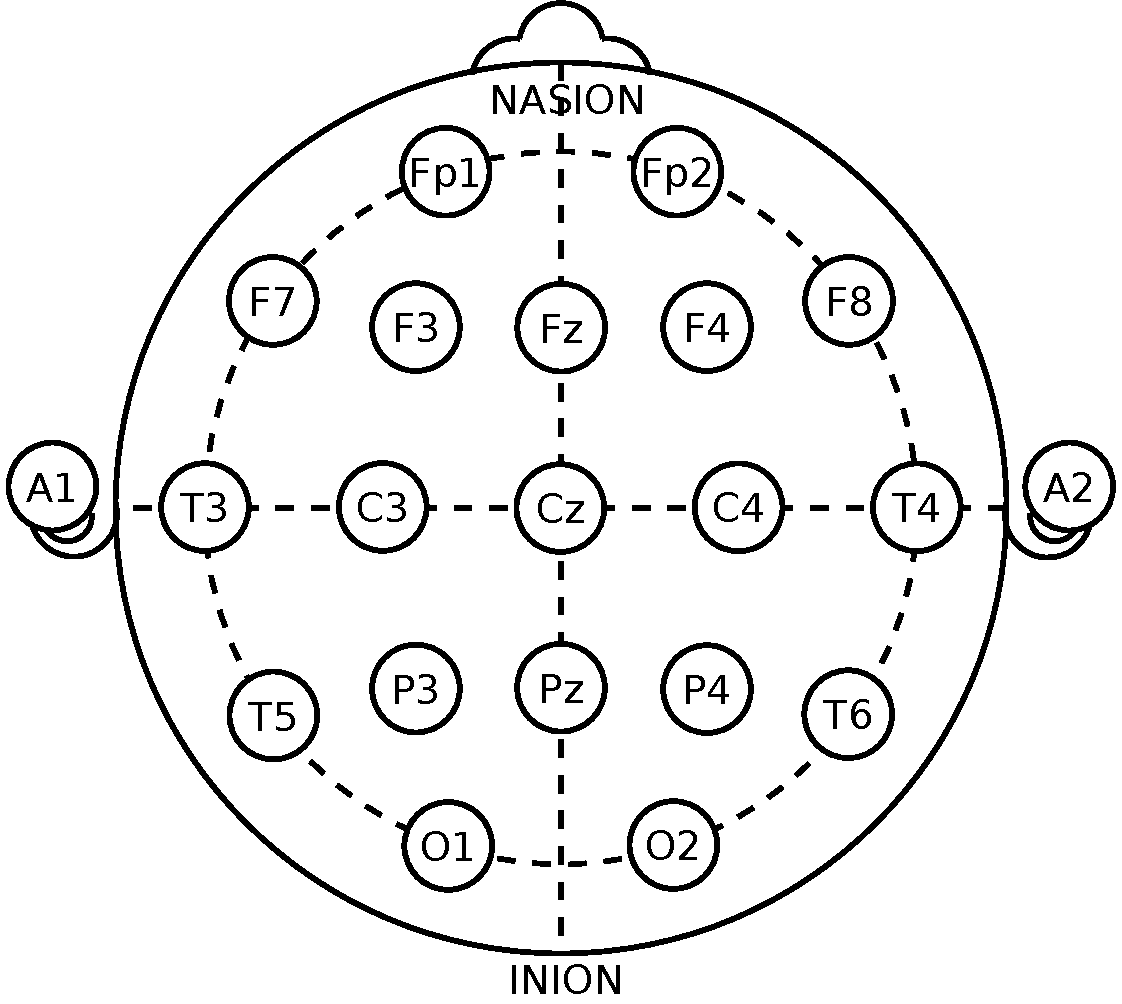
\includegraphics[width=0.8\textwidth]{EEG_Cap.pdf}
    \caption{The standard placement of 21 electrodes according to the International 10-20 system for an electroencephalogram (EEG). The M1 node is equal to A1. Image retrieved from Wikimedia Commons, is in the public domain.}
    \label{fig:eeg_electrodes}
\end{figure}

The AASM \cite{AASM} recommends the following EEG derivations for sleep staging, known as a \textbf{referential montage}:
\begin{itemize}
    \item F4-M1
    \item C4-M1
    \item O2-M1
\end{itemize}
A derivation is a pair of electrodes, for which we measure the difference in voltage between them.
In the above list, the first electrode is placed on the right side of the head, while the second electrode is placed on the left mastoid process.

AASM \cite{AASM} requires that at minimum three derivations are used for sleep staging. Additionally, it prescribes backups, 
if any of nodes fail. For example M1 can be replaced with M2.

It is standard to split EEG data into 30-second epochs. Each epoch is then classified into one of the five sleep stages (W, N1, N2, N3, REM)
If an epoch contains characteristics of multiple stages, the stage that occupies the majority of the epoch is assigned.

Same electrode derivations can be used for children (older than 2 months post-term). However, 
sleep stages can differ. If non-REM sleep is not sufficiently developed (if recording does not contain sleep spindles or
K-complexes), AASM \cite{AASM} recommends using a simplified stage N.
Sleep spindles can appear as early as 6 weeks post-term and are present in all infants by age of 3 months.
However, K-complexes start to appear between 3 and 6 months of age \cite{AASM}. That means, that by age of 
6 months, stage N can be fully divided into N1, N2 and N3 sleep for most children.

For infants (younger than 2 months post-term), AASM \cite{AASM} prescribes a different set of sleep stages:
\begin{itemize}
    \item Wakefulness (W)
    \item Non-REM sleep (N)
    \item REM sleep (R)
    \item Transitional sleep (T)
\end{itemize}
Historically, these stages were often referred to as quiet sleep (N), active sleep (R), and indeterminate sleep (T) \cite{AASM}.

Properties of these stages differ from those in older children and adults. For example, non-REM sleep
can be characterized by Trace alternant pattern - at least 3 alternating runs of high voltage delta waves
lasting 5 to 6 seconds, followed by low voltage theta waves lasting for 4 to 12 seconds.
Non-REM sleep mostly consists of high voltage slow wave activity (delta waves predominating). However,
high voltage slow wave activity can also be present in REM sleep \cite{AASM}. If NREM stage is sufficiently
developed, this stage can already be classified into N1, N2 and N3 sleep. In that case, staging rules for children apply.

On the other hand, REM sleep can be characterized by low voltage mixed frequency activity (delta and theta waves predominating).

To account for the ambiguity of infant sleep patterns, the AASM defines \textbf{Stage T}. This stage is scored when
an epoch contains 3 Non-REM characteristics and 2 REM characteristics, or 2 Non-REM characteristics and 3 REM characteristics \cite{AASM}.
Transitional stage aids the staging process, as sleep stages in infants are not yet fully developed.
\chapter{Related Work} \label{chapter:related_work}
The usage of automatic stage classification tools is an established field of research,
with efforts dating back over half a century. While earlier methods depended on heuristic
algorithms, modern approaches predominantly use machine learning.

One of the first sources from 1970 \cite{FROST197088} used EEG recordings to 
classify sleep stages in real time using specialized hardware. The system 
first preprocessed the signal by amplifying and filtering it, and then 
operated as a so-called \textit{amplitude-weighted, dominant-frequency meter}.
This module evaluated the EEG signal based on its amplitude across three
predefined levels. Depending on which levels were crossed, two different
artificial signals were generated. These were then fed into a resistor-capacitor
integration circuit with a 15-second memory, determining a final voltage
that was used to classify the sleep stage. To identify REM sleep, the device
used an additional EOG channel to detect rapid eye movements.

Similarly, neonatal sleep stage classification attempts date back decades.
An early method from 1987 \cite{HARPER1987379} used 7 cardiac and respiratory measures
of children up to age of 6 months. Using discriminant analysis they developed a model,
for which article reports an overall accuracy of 84.8\%.

However, since the rise of machine learning, more advanced methods have been developed.
Most often, these methods either use EEG or all polysomnography (PSG) signals as input. It is however, most common, 
for these models to learn on a specific demographic. That is, models either see only adult or only
neonatal patients.

\section{Machine Learning Methods for Sleep Stage Classification of Adults}

A random forest classifier was one of the first machine learning models used for sleep stage classification \cite{FRAIWAN201210}.
The model used a single EEG channel represented in the time-frequency domain. Their study consisted of 16 
subjects aged 30 to 75. Researchers tried multiple feature extraction methods and found the 
best results using Continuous Wavelet Transform signal breakdown. Reportedly, 
the model achieved an accuracy of 83\%.

Later, specialized models designed for temporal data were used. A combination of convolutional neural network (CNN)
and long short-term memory (LSTM) network was developed in 2021 \cite{cnnlstm2021}.
Model used three convolutional layers and two LSTM layers and finally a dense layer 
for classification into one of the 5 stages. The model used two EEG channels as input.
The model was tested on 12 subjects, in ages between 21 and 61. The model achieved
an accuracy of 74\%.

Additionally, a transformer-based model called MultiChannelSleepNet was developed \cite{transformersleep2023}.
Rather than operating on raw signals, the model uses time-frequency representations of multiple EEG and EOG
channels: transformer encoders first extract features from each channel independently, and a second, smaller
set of transformer encoders then fuses these into joint features. The model was evaluated on three datasets,
including SleepEDF-78, which contains subjects aged between 25 and 101 years, on which it achieved an accuracy
of 85.0\%.

\section{Machine Learning Methods for Sleep Stage Classification of Infants and Children} 
Similarly to sleep staging for adults, temporal models for neonatal
classification have been developed. Approach from article \cite{neonetalLstm} uses 
a single EEG channel to classify sleep into 3 stages, Awake, Active sleep and Quiet sleep.
All patients were 40 weeks post-conceptional old. Using a bidirectional LSTM network,
and a fully connected classification layer the model achieved an overall accuracy of
96.81\%. Model was evaluated using a 10-fold cross validation \cite{neonetalLstm}.

A CNN model from 2023 aimed to classify sleep 
into Quiet and Non-Quiet stages \cite{neonatalcnn2023}.
The model was trained on EEG data of 19 preterm and term newborns,
using 9 channels as input. The model achieved an accuracy of 94.07\% \cite{neonatalcnn2023}.
The EEG data was first preprocessed into 8 time-domain features and 
four frequency-domain features, which were then used as input into the CNN model.

Similarly to adults, a transformer based model was developed for children sleep staging \cite{transformerinfant2022}.
The architecture used was inspired by Vision Transformers (ViT), which is commonly 
used in image based tasks. However, the architecture was 
modified for multichannel input. An epoch, which consists of 30 seconds of data,
is split into 30 patches, one for each second. This is analogous to tokenization.
From this, the model classifies each epoch into one of the standard 5 stages.
The data consisted of 3.6 million epochs from infants, children and adolescents patient.
Model achieved an overall accuracy of 78.2\%, with 
highest accuracy for patients in the range of 8 to 9 years (85\%) \cite{transformerinfant2022}.
\chapter{Methodology} \label{chapter:methodology}

This chapter details the methodology for classifying sleep stages from EEG recordings, with a specific focus on handling data variations across age groups. 

Section \ref{sec:data_preprocessing} outlines the preprocessing pipeline used to transform heterogeneous raw EEG signals from disparate datasets into standardized time-frequency spectrograms. 

The subsequent sections present four neural network frameworks developed to investigate the optimal method for integrating patient demographic data:
\begin{itemize}
    \item A \textbf{baseline model} (Section \ref{sec:baseline_model}) that relies exclusively on raw EEG signals,
    \item a \textbf{metadata-integrated model} (Section \ref{sec:additional_embeddings}) that injects patient age into the sequence via a learnable classification token,
    \item an \textbf{age-stratified framework} (Section \ref{sec:separate_models}) that routes data to demographically specialized expert models,
    \item a \textbf{fine-tuned model} (Section \ref{sec:finetuning}) that uses transfer learning to adapt a foundational adult-trained model to younger cohorts.
\end{itemize}

\section{Data preprocessing}
\label{sec:data_preprocessing}

To ensure consistency across multiple disparate datasets (e.g., CAP Sleep Database, NCH Sleep DataBank, and Adult High-Density EEG),
a preprocessing pipeline was implemented for each dataset. 
The process transforms raw Electroencephalography (EEG) recordings of 
varying sampling rates and channel configurations into standardized, 
labeled time-frequency representations. 
The pipeline consists of channel standardization, signal filtering,
epoch segmentation, spectrogram generation and data augmentation.

\textbf{Channel Standardization and Bipolar Derivation} \\
Due to inconsistencies in channel and hardware setups across datasets, a channel standardization protocol was applied to match the AASM recommended derivations. The target channels comprise three pairs across the left and right hemispheres: frontal (F3, F4), central (C3, C4), and occipital (O1, O2), referenced to contralateral mastoids or mastoid-adjacent reference points (e.g., M1/M2, A1/A2, or TP9/TP10). 
Depending on the dataset, these channels were either extracted directly, explicitly constructed by subtracting monopolar channels, or resolved using a hierarchical substitution dictionary.
Furthermore, because some datasets or individual recordings contained fewer than the target number of standardized channels, a zero-padding strategy was employed. If an epoch lacked the full channel complement, the missing channels were represented by zero-filled arrays. This ensured a uniform tensor shape for all epochs.

\textbf{Signal Filtering and Resampling} \\
Once standard channels were acquired, the continuous EEG signals were temporally normalized. A band-pass filter with a lower cutoff of $0.3$~Hz and an upper cutoff of $30$~Hz was applied to eliminate baseline drift, low-frequency artifacts, and high-frequency noise. Following filtration, all recordings were resampled to a uniform target sampling frequency of $F_s = 128$~Hz.

\textbf{Segmentation and Sleep Stage Annotation} \\
The continuous recordings were segmented into non-overlapping $30$-second epochs, corresponding to the standard clinical scoring window. Sleep stage annotations from the associated metadata files were parsed and mapped to the standard five-stage classification. Epochs containing invalid sleep stages, or those deviating from the standard $30$-second duration, were discarded.

\textbf{Time-Frequency Feature Extraction} \\
To capture both the spectral and temporal characteristics of the sleep stages, the $30$-second EEG epochs were converted into spectrograms using the short-time Fourier transform (STFT). The STFT was computed individually for each channel with the following parameters:
\begin{itemize}
    \item \textbf{Window length:} $256$ samples ($2$ seconds, after resampling).
    \item \textbf{Overlap:} $128$ samples ($1$ second, equating to a $50\%$ overlap).
\end{itemize}
To reduce computational overhead, the resulting frequency bins were truncated to retain only frequencies below $50$~Hz, a range that comfortably encompasses the $0.3$--$30$~Hz passband established during signal filtering. To handle the high dynamic range of EEG power spectra, the magnitude of the complex STFT output ($|Z_{xx}|$) was subjected to a logarithmic transformation defined by
\begin{equation}
    S = \log(1 + |Z_{xx}|).
\end{equation}
Following this transformation, the spectrograms were subjected to global Z-score normalization. The global mean ($\mu$) and standard deviation ($\sigma$) were computed exclusively across the training set to prevent data leakage. Every spectrogram $S$ was then normalized to have zero mean and unit variance via $S_{norm} = (S - \mu) / \sigma$ before being fed into the neural networks.

\textbf{Data Augmentation via Channel Permutation} \\
To prevent the models from overfitting to specific hardware configurations or fixed channel orderings present in the diverse datasets, a spatial data augmentation technique was applied during the training phase across all experiments. Specifically, the order of the EEG channels within the input tensor was randomly shuffled for every batch. This channel permutation forces the spatial-frequency feature extractor to learn robust, channel-invariant representations rather than relying on fixed spatial indices.

\section{Developed frameworks} \label{sec:developed_frameworks}
\subsection{Baseline model} \label{sec:baseline_model}
Machine learning models are often considered as black boxes, where the inner workings and decision-making processes are not easily interpretable.
Predicting what a machine learning model can learn and what it can interpret from input data alone is complex.
It is possible, the model could learn age-related signal differences (and other factors, such as diseases, gender, etc.), figure out how impactful on sleep classification they are
and use it to predict sleep stages from EEG data alone.
Thus, our first model, which serves as a baseline does not have an insight
on the patient, except for the EEG signal itself.

\begin{figure}
    \begin{center}
        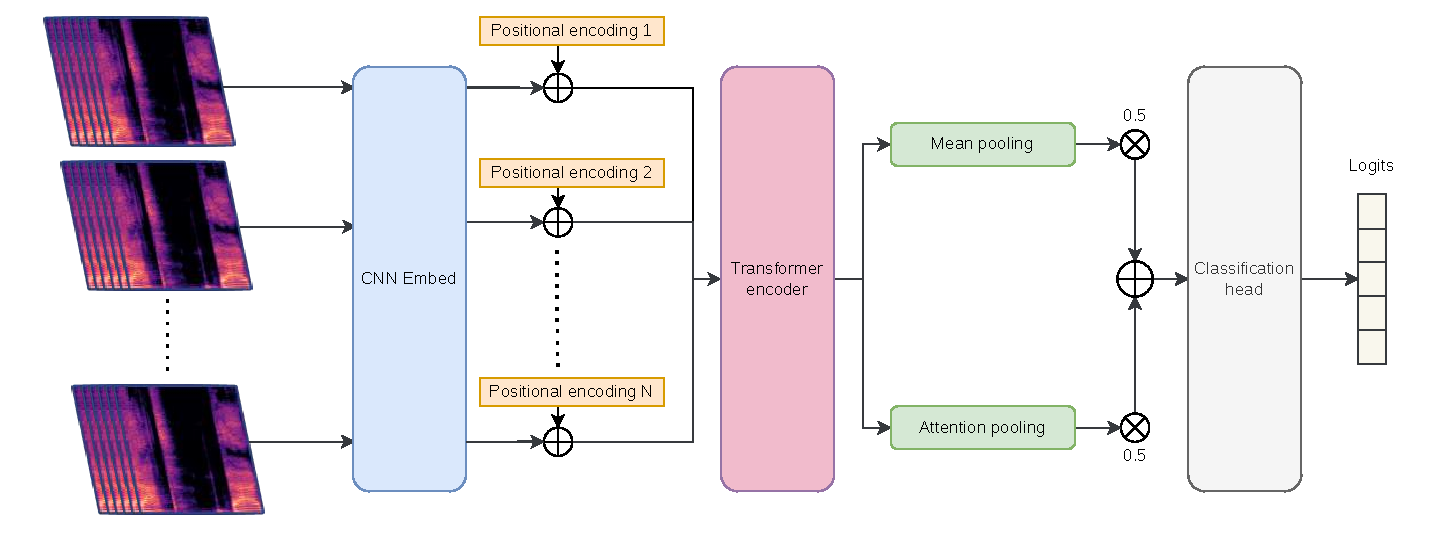
\includegraphics[width=1\linewidth]{models/baseline.drawio.pdf}
    \end{center}
\caption{Baseline model architecture.}
\label{baseline_model_architecture}
\end{figure}

The model consists of two main components: 
\begin{itemize}
    \item A feature extractor, implemented using a convolutional neural network (CNN) architecture, which gets a single epoch as an input,
    \item and a classifier, implemented using a transformer encoder, which predicts the sleep stage based on the embeddings extracted by the feature extractor.
\end{itemize}

\subsubsection*{Feature Extraction}
The feature extractor receives a single epoch (represented as a spectrogram image per EEG channel) as an input and outputs an embedding (array of numbers, representing the learned features of the epoch).
The CNN module consists of two sequential 2D convolutional blocks. Each block utilizes $3 \times 3$ kernels with a stride of 2,
followed by a ReLU activation function and Group Normalization to stabilize training without relying on batch statistics.
The output feature maps are flattened, subjected to Dropout (to mitigate overfitting), and passed through a linear projection layer to
produce a fixed-size token for each epoch.

\subsubsection*{Sequence Modeling and Contextualization}
Because sleep stages are not independent, analyzing epochs in isolation is suboptimal.
Therefore, the network processes a contextual window of 10 consecutive epochs with the goal of predicting the sleep stage of the central epoch.
Each epoch's token has an added learned positional embedding to retain temporal information, allowing the model to understand the order of epochs within the sequence.
These tokens are then passed into a standard Transformer Encoder.
The self-attention mechanism allows the model to weigh the importance of surrounding epochs when evaluating the central epoch.

To aggregate the sequence of contextualized tokens into a single representation for classification, we employ a hybrid pooling strategy. The final representation is an unweighted average of two techniques:
\begin{enumerate}
\item \textbf{Mean Pooling:} The average of all token embeddings across the temporal dimension.
\item \textbf{Attention Pooling:} A learned linear layer projects the tokens to compute raw attention scores. These scores are 
normalized across the temporal dimension using a Softmax function, 
producing weights that sum to one. The pooled representation is the weighted sum (using the computed weights) of the sequence tokens.
\end{enumerate}

Finally, this aggregated representation is passed through a classification head—a multilayer perceptron (MLP) consisting of a linear layer, a ReLU activation, Dropout, and a final linear layer—yielding the logits for the 5 sleep stages.
During training the loss is calculated on the central token using Focal Loss, which is particularly effective for handling class imbalance by down-weighting easy examples and focusing on harder, misclassified examples.

\subsection{Model with additional embeddings} \label{sec:additional_embeddings}

To explicitly account for the age-related domain shifts established in Section \ref{sec:motivation}, we developed a secondary architecture designed to actively integrate patient age metadata into the sequence modeling process.

\begin{figure}
    \begin{center}
        \includegraphics[width=1\linewidth]{models/embeddings.drawio.pdf}
    \end{center}
\caption{Model with additional embeddings.}
\label{embeddings_model_architecture}
\end{figure}

\subsubsection*{Feature Extraction}
The spatial-frequency feature extraction phase of this model is identical to the baseline. The input consisting of 10 consecutive 30-second epochs is passed through the Convolutional Neural Network (CNN) module, producing a sequence of 10 dense feature vectors (tokens).

\subsubsection*{Metadata Integration via a Learnable Class Token}
The primary divergence from the baseline model lies in how the sequence is contextualized. Inspired by architectures such as BERT and ViT, we introduce a learnable classification token (\texttt{[CLS]}). This token acts as a global placeholder that accumulates sequence-wide context during the Transformer's self-attention operations.

To inject the demographic data into the model, the patient's age is first discretized into one of 4 categorical age groups:
\begin{itemize}
    \item infant (0--2 years),
    \item child (2--12 years),
    \item teen (13--18 years),
    \item adult (19+ years).
\end{itemize}

This categorical value is passed through an embedding layer, mapping the age group to a dense vector of the same dimensionality as the EEG tokens. 
Instead of concatenating this metadata to every epoch, the age embedding is combined with the expanded \texttt{[CLS]} token via element-wise addition. Consequently, the \texttt{[CLS]} token becomes an ``age-aware'' global summary token before any sequence processing begins.

\subsubsection*{Sequence Modeling and Representation Extraction}
Once the age-aware \texttt{[CLS]} token is formulated, it is prepended to the sequence of 10 EEG tokens, expanding the overall sequence length to 11. Because the sequence length has increased, the learned positional embedding space is also expanded to 11. These positional embeddings are added to all tokens to establish chronological order, and the combined sequence is fed into the Transformer Encoder.

Unlike the baseline model, which employed a hybrid strategy of Mean and Attention pooling across all epoch tokens to derive a final representation, this updated architecture utilizes a much simpler extraction paradigm. The self-attention mechanism within the Transformer naturally routes relevant temporal and spatial information from the EEG tokens into the prepended \texttt{[CLS]} token. Therefore, upon exiting the Transformer, we discard the 10 epoch tokens and extract only the contextualized \texttt{[CLS]} token.

This single token, which now encapsulates both the contextualized EEG sequence data and the patient's age profile, serves as the definitive global representation. It is passed directly into the MLP classification head to generate the final sleep stage logits.
\subsubsection*{Demographic Batch Balancing}
To ensure the model effectively learns to utilize this age profile across all demographics, we had to address a significant imbalance in the training data. Because adult recordings vastly outnumber pediatric and infant recordings, standard random sampling would bias the network toward adult EEG patterns, severely limiting its ability to learn accurate representations for the younger age cohorts. Therefore, a class-balanced weighted sampling strategy was introduced during the training phase. By assigning sampling probabilities that were inversely proportional to the total number of epochs available for each of the four age groups, we guaranteed that every training batch contained a demographically balanced distribution of data.

\subsection{Separate models (Age-Stratified Framework)} \label{sec:separate_models}

In our third experimental approach, we explore an alternative method for handling demographic variance. Rather than relying on a single, generalized network to learn the complexities of age-related EEG shifts (as attempted in the embedding-based model), we hypothesized that isolating the training data distributions might yield superior results. To test this, we developed an age-stratified routing framework.

\begin{figure}
    \begin{center}
        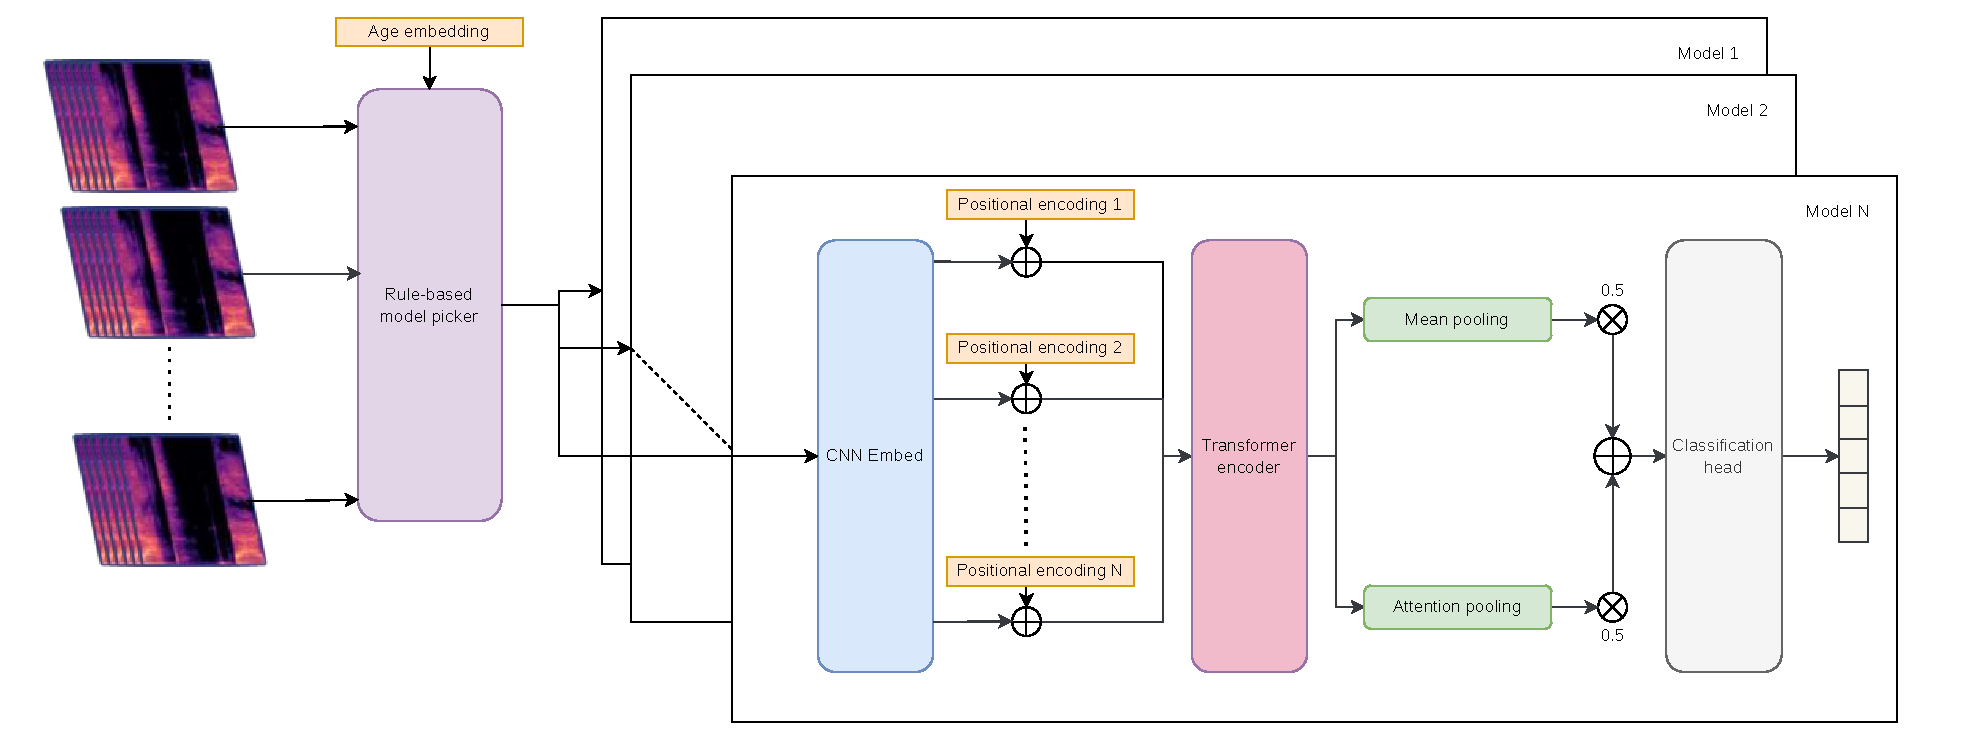
\includegraphics[width=1\linewidth]{models/seperate models.drawio.pdf}
    \end{center}
\caption{Separate trained models per patient metadata.}
\label{embeddings_model_architecture}
\end{figure}

\subsubsection*{Architecture and Data Partitioning}
For this framework, the neural network architecture reverts entirely to the original Baseline model. 
Instead of altering the model's internal architecture, we altered the training data distribution.
The global training dataset was partitioned into four age groups defined in previous section.

We independently initialized and trained four distinct instances of the baseline model, one for each demographic cohort. Consequently, each model acts as a demographic expert, highly specialized in the specific characteristics of its respective age group.

\subsection{Fine-tuned model} \label{sec:finetuning}
In our fourth and final experimental approach, we explore a transfer
learning paradigm. Typically, in physiological datasets, data from
adult cohorts is vastly more abundant than data from pediatric or
infant cohorts. To leverage this imbalance, we hypothesized that a model
could first learn foundational, universal EEG characteristics from
the largest demographic group and later learn age-specific patterns
on smaller specific datasets.

The foundation of this framework is the adult specific model from 
section \ref{sec:separate_models}.
We prepare the trained model for fine-tuning on the remaining age groups (infants, children, and teens). Rather than updating the entire network during fine-tuning—which risks catastrophic forgetting and overfitting on smaller pediatric cohorts—we employ a selective partial layer-freezing strategy. 

Specifically, the gradient updates are configured as follows:
\begin{itemize}
    \item \textbf{Frozen Feature Extractor:} The parameters of the Convolutional Neural Network are completely frozen. The underlying assumption is that low-level spectrogram features extracted by the CNN are similar across all ages. Freezing this module preserves these generalized feature representations.
    \item \textbf{Unfrozen Sequence Modeling:} The Transformer encoder layers are unfrozen. While low-level EEG features may be universal, the temporal dynamics of sleep, such as the duration of sleep cycles, and transition probabilities, change significantly from infancy to adulthood. Unfreezing the Transformer allows the self-attention mechanism to adapt to these age-specific sequential patterns.
    \item \textbf{Unfrozen Classification Head:} The final MLP mapping the pooled representation to the 5 sleep stages is also unfrozen. This ensures the decision boundaries can shift to accommodate the updated temporal representations.
\end{itemize}

This approach acts as a hybrid between the generalized Baseline model and the specialized framework. By isolating the layers responsible for temporal context and classification, this framework aims to retain the robust, generalized feature-extraction capabilities learned from a massive adult dataset, while adapting only the reasoning modules to other age groups.
\chapter{Evaluation}

This chapter presents the evaluation framework of our proposed automated sleep staging architectures.
We first establish the capabilities and limitations of a baseline generalist network,
highlighting its vulnerability to missing data and developmental EEG variations.
Subsequent experiments systematically address these challenges through demographic-conditioning,
age-specific model partitioning, and transfer learning, ultimately concluding with a benchmark comparison
against a widely established, off-the-shelf model Yet Another Spindle Algorithm (YASA).

\section{Experiment 1: Baseline Architecture}
The first phase of our evaluation aimed to establish the predictive capabilities of the base network without the inclusion of any demographic information. This baseline serves as a benchmark to assess both the raw learning capacity of the model and its vulnerabilities when we subject it to suboptimal clinical conditions.

\subsection{Hyperparameter Optimization}
To determine the optimal configuration for the baseline model, we conducted a series of grid search experiments over an extensive hyperparameter space. We iteratively explored various combinations of learning rates, the number of Transformer encoder layers, dropout probabilities, and batch sizes. We trained all configurations for a maximum of 15 epochs and evaluated them based on their validation performance.
Following the hyperparameter search, we identified the best-performing baseline configuration as:
\begin{itemize}
    \item \textbf{learning rate:} $5 \times 10^{-5}$ (with a weight decay of $1 \times 10^{-5}$),
    \item \textbf{transformer layers:} 2,
    \item \textbf{attention heads:} 8,
    \item \textbf{embedding size:} 64,
    \item \textbf{dropout:} 0.4,
    \item \textbf{batch size:} 16
\end{itemize}
During training, we employed a learning rate scheduler to gradually decay the learning rate, and implemented early stopping to halt training if the validation loss ceased to improve, thereby preventing overfitting.

\subsection{Results and Limitations}
We evaluated the performance of the baseline model under two main configurations: utilizing all 6 EEG channels and utilizing a reduced set of 3 EEG channels. We also analyzed the model's predictive capabilities across four distinct age cohorts (as we defined previously in Section \ref{sec:additional_embeddings}).

\subsubsection*{Full Model (6 Channels)}
We initially trained and evaluated the model on the complete set of 6 EEG channels. The training converged successfully, triggering early stopping at epoch 10 (we observed the lowest validation loss at epoch 5). On the test set, this full-resolution model achieved an overall accuracy of 75.01\%, and a Cohen's Kappa of 0.668 (see Table~\ref{tab:overall_results}). 

As we detail in Table~\ref{tab:age_group_results}, the model's performance varied significantly among different age groups. It performed best on adults (accuracy of 76.76\%) and worst on teenagers (accuracy of 66.13\%).

\subsubsection*{Robustness to Missing Channels}
In clinical practice, missing data or detached sensors are common issues that disrupt the expected acquisition and spatial resolution of EEG recordings. To test the robustness of the 6-channel model against missing data, we evaluated the already-trained model using only the first 3 channels, effectively simulating the loss of 3 sensors during inference. 
While a channel dropout of this magnitude is unlikely in standard practice, this extreme case serves as a test of the model's resilience.

This simulated sensor loss exposed a major limitation in the baseline architecture, causing a severe degradation in overall performance. The accuracy dropped by nearly 13 percentage points to 62.16\%, and Cohen's Kappa fell to 0.506. We observed the most catastrophic decline in the children cohort, where accuracy plummeted from an initial 75.17\% to a mere 46.58\%. This brittle behavior suggests that the baseline model over-relies on strict cross-channel dependencies and struggles to generalize when missing channels compromise those inputs.

\subsubsection*{Reduced Channel Model (3 Channels)}
To determine if the model could effectively learn stage-discriminative features from a limited spatial resolution from scratch, we trained a second baseline model entirely on 3 channels using the same optimal hyperparameters. Early stopping concluded this training at epoch 7.

This natively trained 3-channel model achieved an overall accuracy of 73.35\%, and a Cohen's Kappa of 0.648. These results indicate that while the 3-channel data contains slightly less predictive information overall compared to the 6-channel data, training the model directly on the reduced channel set successfully circumvents the catastrophic performance drop we observed during the robustness test.

Interestingly, for teenagers, the 3-channel model performed much better than the 
6-channel baseline (81.28\% vs. 66.13\%). We speculate this happens because the 
dataset consists mostly of adults. 
When we provide all 6 channels, the model learns the exact sensor patterns typical of 
adult brains. However, because adolescent brains are still developing, teenage sleep 
signals spread across the head differently than adult signals. In the 6-channel model, 
these spatial differences confuse the network and hurt teenage performance.
Reducing the input down to 3 channels solves this issue. With fewer sensors to rely on, 
the network stops depending on adult-specific sensor layouts. Instead, the reduced input 
forces the network to focus on the core shape and timing of the sleep waves themselves. 
Because teenagers and adults share these core wave patterns, the 3-channel model generalizes 
much better to teenagers.
\begin{table}[ht]
\centering
\caption{\textbf{Baseline Model Overall Performance.} This table presents the evaluation metrics across three different channel configurations. It highlights the baseline's vulnerability to missing channels during inference and its subsequent recovery when we natively train it on a reduced channel set.}
\label{tab:overall_results}
\begin{tabular}{l c c}
\toprule
\textbf{Model Evaluation Setup} & \textbf{Accuracy} & \makecell[c]{\textbf{Cohen's}\\\textbf{Kappa}} \\
\midrule
Trained on 6 ch, Evaluated on 6 ch & 75.01\% & 0.668 \\
Trained on 6 ch, Evaluated on 3 ch & 62.16\% & 0.506 \\
Trained on 3 ch, Evaluated on 3 ch & 73.35\% & 0.648 \\
\bottomrule
\end{tabular}
\end{table}

\begin{table}[ht]
\centering
\caption{\textbf{Performance Breakdown by Age Cohort.} This table details the accuracy, and Cohen's Kappa scores across four distinct age groups for each channel setup. It illustrates the severe impact of simulated missing data on younger cohorts and the unexpectedly improved generalization for teenagers when we train the model on fewer channels.}
\label{tab:age_group_results}
\resizebox{\textwidth}{!}{%
\begin{tabular}{l c c | c c | c c}
\toprule
& \multicolumn{2}{c|}{\textbf{Evaluated on 6 ch}} & \multicolumn{2}{c|}{\textbf{Evaluated on 3 ch (Missing Data)}} & \multicolumn{2}{c}{\textbf{Trained \& Evaluated on 3 ch}} \\
\cmidrule(lr){2-3} \cmidrule(lr){4-5} \cmidrule(l){6-7}
\textbf{Age Group} & \textbf{Accuracy} & \textbf{Kappa} & \textbf{Accuracy} & \textbf{Kappa}& \textbf{Accuracy} & \textbf{Kappa} \\
\midrule
Adults   & 76.76\% & 0.684 & 73.49\% & 0.641 & 75.85\% & 0.671 \\
Teenagers& 66.13\% & 0.515 & 71.43\% & 0.613 & 81.28\% & 0.733 \\
Children & 75.17\% & 0.640 & 46.58\% & 0.299 & 67.30\% & 0.531 \\
Infants  & 73.14\% & 0.646 & 51.45\% & 0.352 & 71.48\% & 0.623 \\
\bottomrule
\end{tabular}%
}
\end{table}

\FloatBarrier
\section{Experiment 2: Age-Conditioned Model}
\label{sec:exp2_data}
The baseline results showed that the model performs inconsistently across different age groups and easily breaks down whenever EEG channels are missing. We hypothesized that forcing the baseline network to implicitly deduce a patient’s developmental stage from raw EEG signals caused it to over-rely on brittle, age-specific spatial topographies. To alleviate this, Experiment 2 introduces a demographic prior: an additional embedding we provide as input to explicitly inform the model of the patient's age group.

\subsection{Dataset Distribution and Setup}
Before evaluating the age-conditioned model, it is crucial to outline the underlying data distribution across the cohorts, as this massively impacts the generalist network's bias. We distributed the total training dataset as follows:
\begin{itemize}
    \item \textbf{adults:} 167,501 samples,
    \item \textbf{teenagers:} 54,267 samples,
    \item \textbf{children:} 7,429 samples,
    \item \textbf{infants:} 81,001 samples.
\end{itemize}
Given this extreme imbalance, models we train on the aggregate dataset are inherently biased toward adult representations. 

To conduct this experiment, we concatenated an age-embedding vector to the temporal feature representations before the Transformer encoder layers. Similar to Experiment 1, we performed an extensive hyperparameter grid search. We trained the models for up to 15 epochs with early stopping. The optimal configurations we selected for final evaluations differed slightly depending on the spatial resolution we modeled:
\begin{itemize}
    \item \textbf{6-Channel Setup:} Learning rate of $5 \times 10^{-5}$, batch size of 32, embedding size of 64, 4 attention heads, 3 Transformer layers, and a dropout rate of 0.4.
    \item \textbf{3-Channel Native Setup:} Learning rate of $5 \times 10^{-5}$, batch size of 16, embedding size of 64, 4 attention heads, 4 Transformer layers, and a higher dropout rate of 0.5.
\end{itemize}

\subsection{Results and Limitations}

\subsubsection*{Full Model (6 Channels)}
The overall accuracy of the natively trained 6-channel age-conditioned model was 74.78\% (Cohen's Kappa was 0.666), which is marginally lower than the overall performance of the non-conditioned baseline (75.01\%). However, inspecting the breakdown in Table~\ref{tab:exp2_age_group_results} reveals a much more balanced model across the demographics. 

By offloading the task of age deduction to the explicit embedding, the network's performance on underrepresented or morphologically distinct groups improved notably. For Teenagers, accuracy jumped from 66.13\% in the baseline to 70.89\%. The Children cohort improved from 75.17\% to 76.18\%, and Infants improved slightly from 73.14\% to 73.79\%. This balance came at a small cost to the dominant Adult cohort, which dropped from 76.76\% to 75.36\%.

\subsubsection*{Robustness to Missing Channels}
We observed the most significant impact of the demographic prior during the missing data simulation. When we evaluated the 6-channel age-conditioned model on only 3 channels, overall accuracy dropped from 74.78\% to 71.46\%. 

While still a degradation, this $\sim$3.3 percentage point drop is drastically less severe than the catastrophic 13-point drop we observed in the baseline (Experiment 1). Crucially, the model successfully protected the highly vulnerable Children cohort. In the baseline experiment, simulating sensor loss caused the Children cohort's accuracy to crash to an unusable 46.58\%. With the age embedding included, the same missing-channel evaluation maintained an accuracy of 70.61\%. It seems that explicitly providing the age group acts as a powerful regularizer, preventing the network from memorizing brittle spatial layouts as a proxy for the patient's developmental stage.

\subsubsection*{Reduced Channel Model (3 Channels)}
When we trained the age-conditioned model natively on 3 channels, it achieved an overall accuracy of 73.08\% (Cohen's Kappa was 0.643). Interestingly, native 3-channel training further improved performance for the Teenagers (77.38\%) and Infants (73.83\%) cohorts compared to the 6-channel conditioned model, reinforcing the finding that restricting spatial dimensions can act as a form of regularization that aids generalization for certain non-adult cohorts.

\begin{table}[ht]
\centering
\caption{\textbf{Demographic Prior Impact by Age Group.} This table illustrates the conditioned model's metrics across the four developmental stages. It highlights how the explicit age embedding balances predictive accuracy across demographic groups and shields the vulnerable children cohort from catastrophic failure during data loss.} \label{tab:exp2_age_group_results}
\resizebox{\textwidth}{!}{%
\begin{tabular}{l c c | c c | c c}
\toprule
& \multicolumn{2}{c|}{\textbf{Evaluated on 6 ch}} & \multicolumn{2}{c|}{\textbf{Evaluated on 3 ch (Missing Data)}} & \multicolumn{2}{c}{\textbf{Trained \& Evaluated on 3 ch}} \\
\cmidrule(lr){2-3} \cmidrule(lr){4-5} \cmidrule(l){6-7}
\textbf{Age Group} & \textbf{Accuracy} & \textbf{Kappa} & \textbf{Accuracy} & \textbf{Kappa} & \textbf{Accuracy} & \textbf{Kappa} \\
\midrule
Adults    & 75.36\% & 0.663 & 73.77\% & 0.641 & 71.82\% & 0.611 \\
Teenagers & 70.89\% & 0.589 & 71.43\% & 0.588 & 77.38\% & 0.680 \\
Children  & 76.18\% & 0.655 & 70.61\% & 0.584 & 75.15\% & 0.641 \\
Infants   & 73.79\% & 0.653 & 68.62\% & 0.585 & 73.83\% & 0.654 \\
\bottomrule
\end{tabular}%
}
\end{table}

\begin{figure}[htbp]
    \centering
    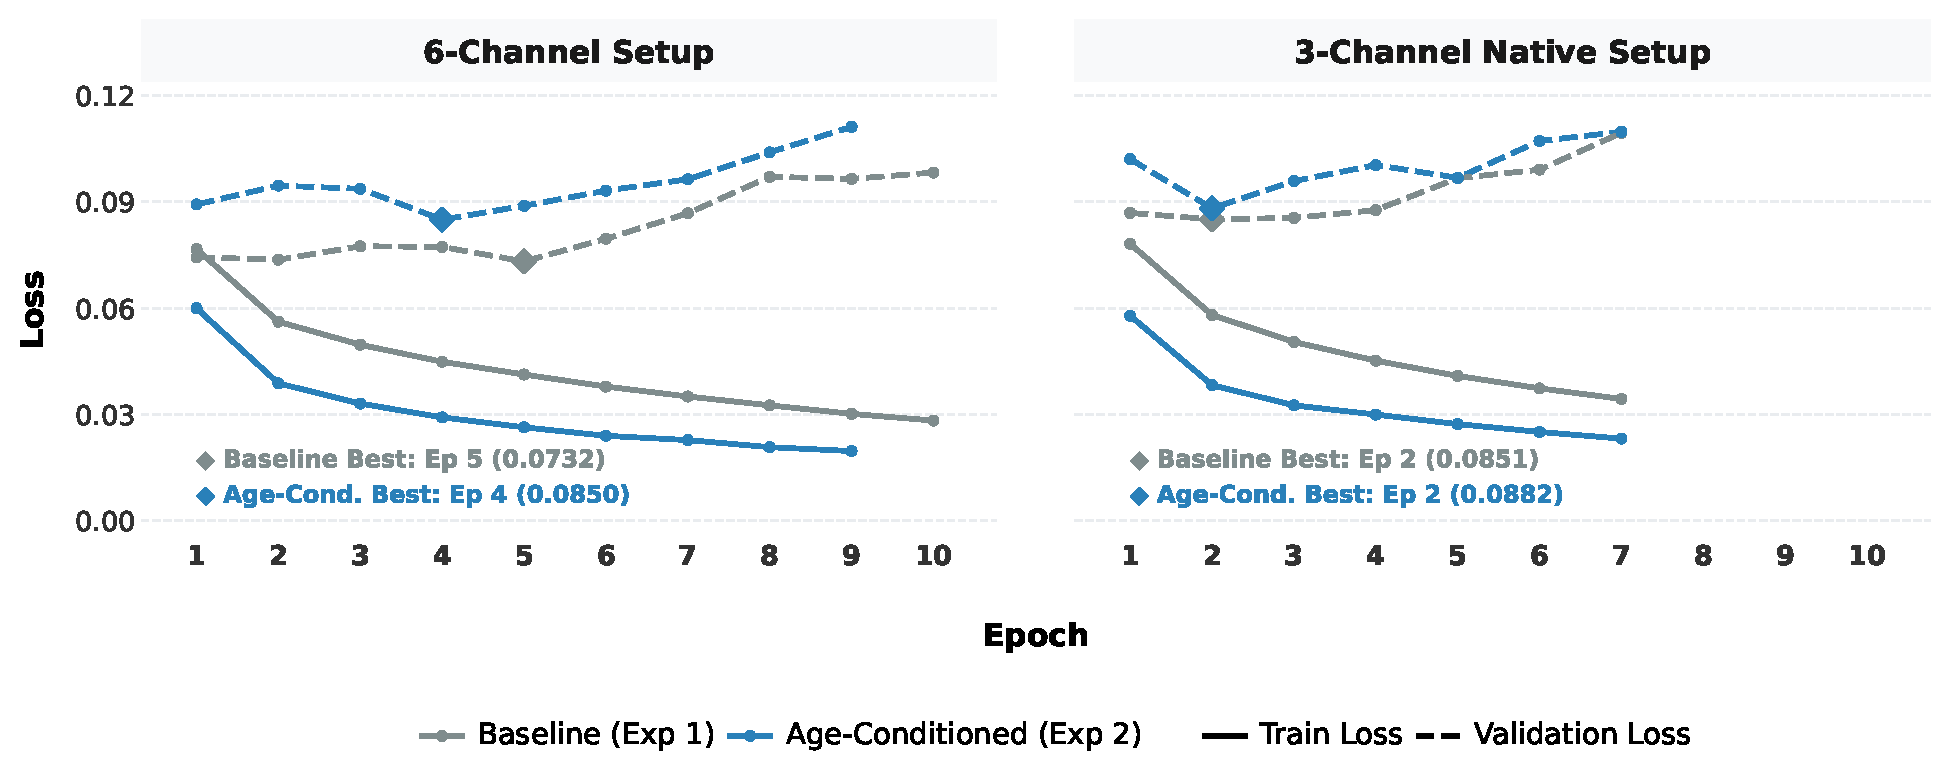
\includegraphics[width=\textwidth]{fig_loss_generalist.pdf}
\caption{\textbf{Training and Validation Loss Curves for Generalist Models (Experiments 1 and 2).} Direct comparison of convergence and generalization across the 6-channel and native 3-channel setups, with diamonds marking the best validation checkpoints. In both architectures, training loss decreases steadily while validation loss reaches its minimum in early epochs before rising due to overfitting, motivating early stopping.}    \label{fig:exp1_exp2_loss}
\end{figure}

\FloatBarrier
\section{Experiment 3: Age-Specific Models}
While the age-conditioned model (Experiment 2) successfully mitigated spatial brittleness and balanced cohort metrics, it still processed all demographics through shared temporal weights. We hypothesized that the generalist model might still be underfitting purely demographic-specific patterns. To test this, we completely partitioned the dataset into the four distinct age cohorts and trained dedicated, age-specific models for each group. 

\subsection{Setup}
We trained each model independently using the optimal hyperparameters we established in the baseline experiment. We employed early stopping based on validation loss to prevent overfitting. As we detailed previously in Section \ref{sec:exp2_data}, the volume of training data varies significantly across the cohorts (ranging from over 167,000 samples for Adults to merely 7,429 for Children). This severe discrepancy naturally influences both the convergence speed and the generalization capabilities of the resulting independent networks.

\subsection{Results and Limitations}
As in the previous experiments, we evaluated the performance of the age-specific models under two spatial resolutions: utilizing the full 6-channel configuration and simulating a modality mismatch by feeding only 3 channels into the 6-channel trained model. Finally, we evaluated natively trained 3-channel models.

\subsubsection*{Full Model (6 Channels)}
By isolating the age groups, the specialized models yielded mixed results when compared to the generalist baseline. We observed the most profound improvement in the Teenagers cohort, where accuracy surged from 66.13\% in the unconditioned baseline model to 83.38\% (Cohen's Kappa was 0.768). The Infants model also saw a slight improvement, achieving an accuracy of 74.87\% compared to the baseline's 73.14\%. 

Conversely, the model trained specifically on the Adults cohort actually saw a slight decrease in accuracy (75.74\% compared to the baseline's 76.76\%), suggesting that the generalist model benefited from the massive aggregate dataset for this dominant group. The Children cohort performed significantly worse than the generalist setups (70.37\% accuracy compared to 76.18\% in the conditioned model). This degradation is directly attributable to the exceptionally small training set for this specific age group, which proved insufficient for an isolated 6-channel model to learn robust stage-discriminative features without overfitting.

\subsubsection*{Robustness to Missing Channels}
To evaluate robustness against sensor loss, we tested the specialized 6-channel models using only 3 channels. Similar to the unconditioned baseline experiment, spatial reduction exposed significant vulnerabilities, though the severity varied substantially by age group. 

The Adults model proved relatively robust, suffering only a moderate drop in accuracy to 73.09\% (down from 75.74\%). The Teenagers model also demonstrated reasonable resilience, dropping to 75.66\%. In stark contrast, the Infants model fell by nearly 11 points to 64.27\%. The most catastrophic failure occurred in the data-starved Children model, where accuracy plummeted to a mere 34.69\% (Cohen's Kappa was 0.188). This demonstrates that without sufficient training volume, an isolated network completely over-leverages highly specific spatial patterns that, when missing, effectively reduce the model's predictions to random guessing.

\subsubsection*{Reduced Channel Model (3 Channels)}
To ascertain whether we could avoid the missing-channel collapse, we natively trained and evaluated age-specific models entirely on the reduced 3-channel setup. Training directly on the restricted spatial resolution successfully restored performance across all cohorts compared to the simulated missing-data scenario.

For Adults, Teenagers, and Infants, the natively trained 3-channel models performed remarkably close to their 6-channel counterparts (achieving accuracies of 75.55\%, 82.61\%, and 73.59\%, respectively). This indicates that we preserve the core sleep staging information even with fewer sensors. 

\begin{table}[ht]
\centering
\caption{\textbf{Age-Specific Model Performance.} This table displays the evaluation metrics for networks trained exclusively on isolated demographic cohorts. It highlights the significant accuracy gains for teenagers, as well as the extreme vulnerability of the children model which we trained on a much smaller dataset when we subjected it to simulated sensor loss.} \label{tab:age_specific_results}
\resizebox{\textwidth}{!}{%
\begin{tabular}{l c c | c c | c c}
\toprule
& \multicolumn{2}{c|}{\textbf{Evaluated on 6 ch}} & \multicolumn{2}{c|}{\textbf{Evaluated on 3 ch (Missing Data)}} & \multicolumn{2}{c}{\textbf{Trained \& Evaluated on 3 ch}} \\
\cmidrule(lr){2-3} \cmidrule(lr){4-5} \cmidrule(l){6-7}
\textbf{Age Group} & \textbf{Accuracy} & \textbf{Kappa} & \textbf{Accuracy} & \textbf{Kappa} & \textbf{Accuracy} & \textbf{Kappa} \\
\midrule
Adults    & 75.74\% & 0.670 & 73.09\% & 0.633 & 75.55\% & 0.668 \\
Teenagers & 83.38\% & 0.768 & 75.66\% & 0.648 & 82.61\% & 0.756 \\
Children  & 70.37\% & 0.573 & 34.69\% & 0.188 & 67.18\% & 0.502 \\
Infants   & 74.87\% & 0.665 & 64.27\% & 0.523 & 73.59\% & 0.648 \\
\bottomrule
\end{tabular}%
}
\end{table}

\FloatBarrier
\section{Experiment 4: Fine-Tuning Pre-Trained Adult Models on Younger Cohorts}

Findings from Experiment 3 highlighted a critical challenge in modeling pediatric and adolescent sleep: extreme data imbalance across demographics. The specialized models for younger cohorts (particularly Children, with only 7,429 training samples) suffered from insufficient data, limiting their ability to learn robust, generalized representations from scratch. To address this, we theorized that we could leverage the vast amount of adult data (over 167,000 samples) to learn foundational sleep features, which we could then adapt to younger demographics.

\subsection{Setup and Methodology}
In this experiment, we employed a transfer learning approach. We utilized both the 6-channel and 3-channel models we trained exclusively on Adults (from Experiment 3) as our base networks. 

We subsequently fine-tuned these pre-trained networks independently on the respective datasets for teenagers, children, and infants. To comprehensively evaluate the models and assess robustness to sensor loss, we evaluated the fine-tuned 6-channel models twice: once on the full 6 channels, and once using only 3 channels to simulate missing data. At the same time, we evaluated the fine-tuned 3-channel models natively on 3 channels. The fine-tuning process retained the optimal hyperparameter configuration we established earlier (learning rate of $5 \times 10^{-5}$, batch size of 16, and dropout of 0.4), utilizing early stopping based on validation loss.

\subsection{Results and Discussion}

Table~\ref{tab:transfer_learning_comparison_all} details the performance of the transfer learning approach across the three evaluation setups. 

\begin{table}[ht]
\centering
\caption{\textbf{Transfer Learning Performance Across Target Demographics.} This table presents the evaluation metrics for each cohort after fine-tuning adult pre-trained base models. It shows that adult priors work better on teenage cohorts which are similar to the adult population and provide regularization that substantially buffers against performance collapse during sensor loss.} \label{tab:transfer_learning_comparison_all}\resizebox{\textwidth}{!}{%
\begin{tabular}{l c c | c c | c c}
\toprule
& \multicolumn{2}{c|}{\textbf{TL (Trained 6ch $\rightarrow$ Eval 6ch)}} & \multicolumn{2}{c|}{\textbf{TL (Trained 6ch $\rightarrow$ Eval 3ch)}} & \multicolumn{2}{c}{\textbf{TL (Trained 3ch $\rightarrow$ Eval 3ch)}} \\
\cmidrule(lr){2-3} \cmidrule(lr){4-5} \cmidrule(l){6-7}
\textbf{Target Age Group} & \textbf{Accuracy} & \textbf{Kappa} & \textbf{Accuracy} & \textbf{Kappa} & \textbf{Accuracy} & \textbf{Kappa} \\
\midrule
Teenagers & 83.63\% & 0.768 & 80.62\% & 0.731 & 82.26\% & 0.751 \\
Children  & 67.22\% & 0.525 & 57.27\% & 0.413 & 69.99\% & 0.559 \\
Infants   & 71.05\% & 0.616 & 63.71\% & 0.515 & 72.41\% & 0.632 \\
\bottomrule
\end{tabular}%
}
\end{table}

\subsubsection*{Overall Performance vs. Training from Scratch}
Contrary to initial expectations, transfer learning did not uniformly improve absolute peak performance compared to the models 
we trained from scratch in Experiment 3. When we evaluated the full 6-channel models, the fine-tuned network for Teenagers achieved a 
marginal improvement, reaching 83.63\% compared to its from-scratch counterpart (83.38\%). However, the fine-tuned models for Children
(67.22\%) and Infants (71.05\%) underperformed their from-scratch baselines (70.37\% and 74.87\%, respectively). This suggests that
while adult priors provide a strong initialization that transfers effectively to adolescents, heavily anchoring the weights in adult
spatial-temporal features may slightly restrict the model from perfectly converging on the more distinct, native EEG morphologies of
early developmental pediatric cohorts. This is somewhat sensible as sleep patterns go through quite large changes, from birth and into adulthood. \todo{ukradeno iz tvojega komentarja :) se mi zdi da je to samo po sebi dovolj dobra hipoteza.}

\subsubsection*{Mitigating Catastrophic Degradation}
Where transfer learning demonstrated profound clinical value was in improving robustness for data-starved demographics. In Experiment 3, the from-scratch 6-channel Children model suffered a catastrophic collapse to 34.69\% accuracy when we evaluated it on 3 channels. In stark contrast, the transfer-learned 6-channel model maintained a much more stable 57.27\% accuracy under the exact same missing-data simulation. By grounding the network in generalized spatial priors we learned from the massive adult dataset, the fine-tuned model avoids over-leveraging spatial correlations, significantly buffering against random guessing during sensor loss.

\subsubsection*{3-Channel Transfer Learning as Regularization}
Interestingly, for the Infant cohorts, fine-tuning the natively 3-channel adult model yielded better overall accuracy (72.41\%) than fine-tuning the full 6-channel model (71.05\%). This reinforces a finding we observed in Experiment 3: a reduced spatial resolution effectively acts as a form of architectural regularization. When we adapt learned weights across demographic domains, restricting the spatial feature space prevents the transfer of overly rigid, adult-specific spatial patterns, ultimately improving generalization on the younger target domains.

\begin{figure}[p]
    \centering
    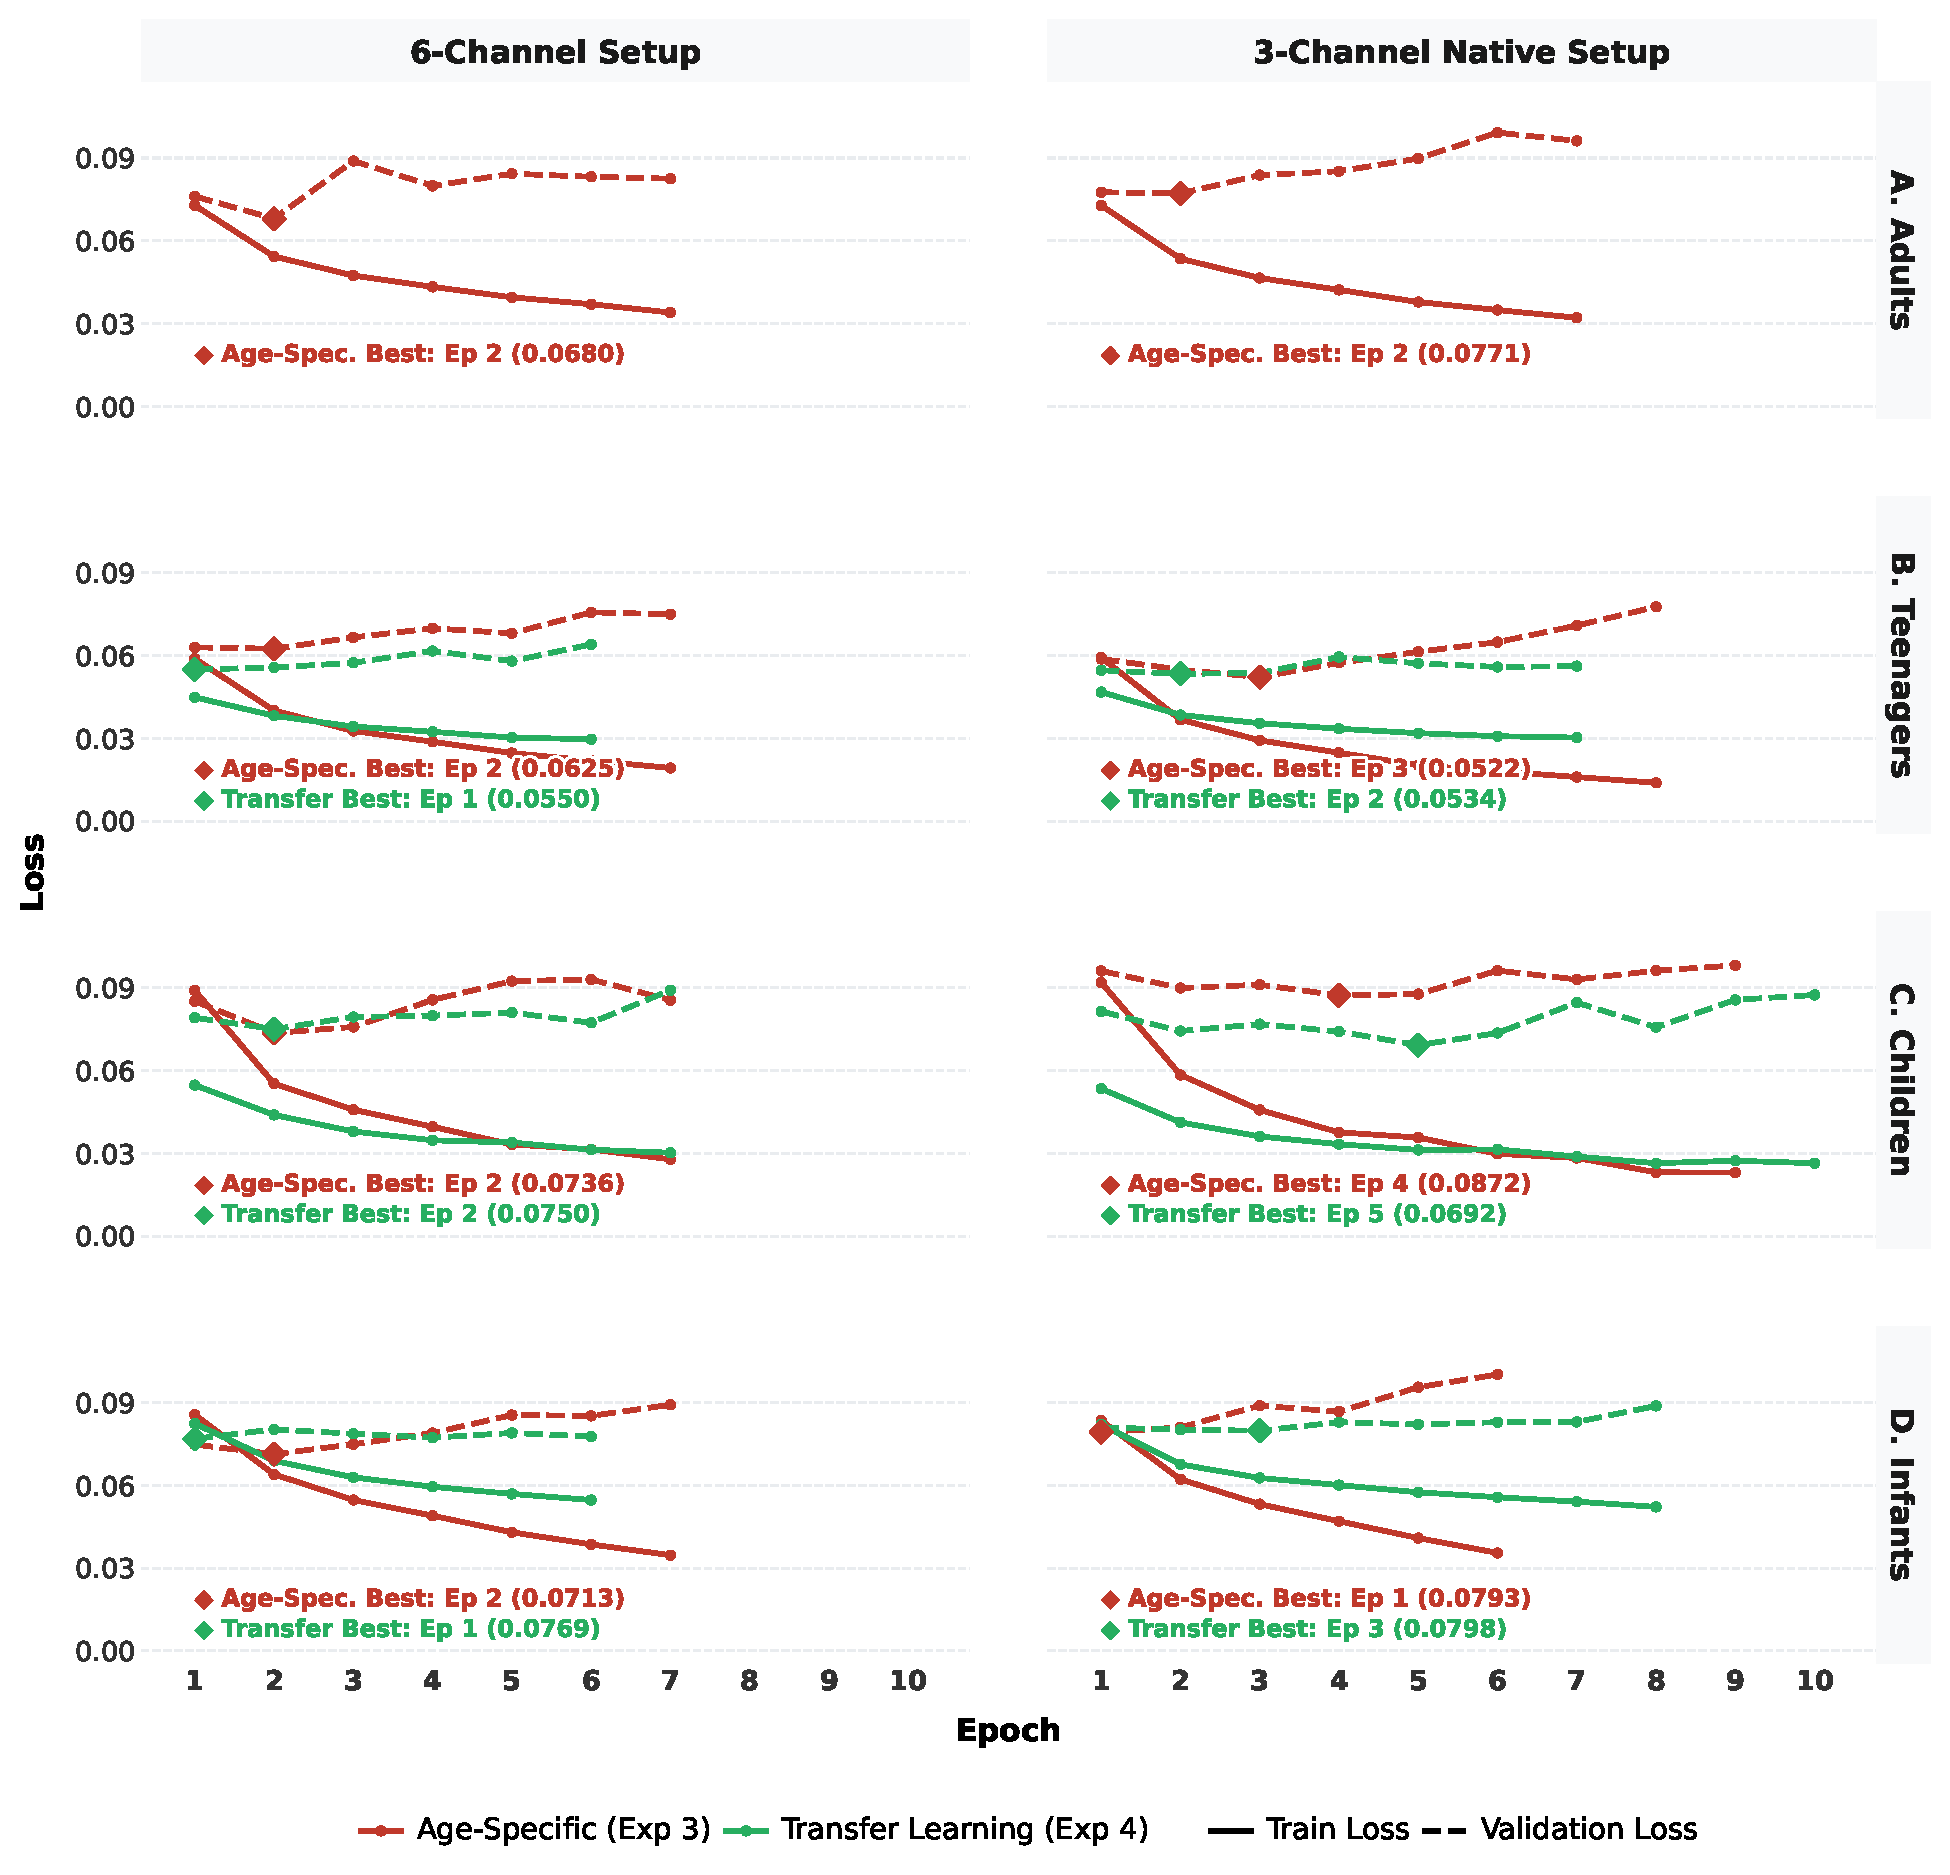
\includegraphics[width=\textwidth]{fig_loss_age_vs_tl.pdf}
    \caption{\textbf{Training and Validation Loss Curves for Age-Specific and Transfer Learning Models (Experiments 3 and 4).} Fine-tuning adult priors (green) yields lower initial training loss across younger cohorts compared to training from scratch (red).}
    \label{fig:exp3_exp4_loss}
\end{figure}

\FloatBarrier

\section{Experiment 5: Comparison with an Established Classification Model (YASA)} \label{sec:yasa_comparison}
YASA (Yet Another Spindle Algorithm) \cite{VallatWalker2021} is a popular, publicly available open-source tool for automated sleep staging. In this section, we evaluate how our proposed architectures compare to this highly established, off-the-shelf model. 

\subsection{Setup and Methodology}
We evaluated the YASA model on a specific subset of our data due to differing input requirements.
While our proposed models independently process isolated 30-second
multi-channel spectrograms, YASA operates on a single EEG channel and relies on temporal context across
surrounding epochs, requiring continuous sleep recordings as input. Our model is therefore more flexible in its input requirements,
as we can always compute spectrograms from raw EEG recordings, whereas we cannot reconstruct raw EEG from spectrograms due to the loss of phase information.
We sourced all recordings used for this comparative baseline from the NCH Sleep DataBank \cite{NCHSleep}.

Furthermore, YASA's feature extraction incorporates patient sex as a demographic input. Because explicit sex metadata was unavailable for this specific evaluation subset, we adopted an optimistic evaluation protocol: we evaluated each recording twice—once configured as male and once as female—and retained the higher-performing outcome. This ensures an upper-bound estimate of YASA's predictive capability on our dataset.

We calculated the accuracy of the YASA model for each age group, reporting results as the mean accuracy across the individual recordings alongside the standard deviation. We summarize the details of this evaluation subset—including the number of full recordings and total extracted 30-second epochs per demographic—as well as the resulting model performance, in Table~\ref{tab:yasa_results}.

\begin{table}[ht]
\centering
\caption{\textbf{YASA Benchmark Performance Across Age Cohorts.} This table summarizes the recording counts, total epoch volumes, and mean classification accuracy for the off-the-shelf YASA model on the NCH Sleep DataBank subset. It reveals a steep developmental degradation, demonstrating that adult-centric staging features struggle to generalize down to infant cohorts.}
\label{tab:yasa_results}
\begin{tabular}{l c c c}
\toprule
\textbf{Age Group} & \textbf{Recordings ($n$)} & \textbf{Epochs} & \textbf{Accuracy (Mean $\pm$ SD)} \\
\midrule
Adults    & 55 & 52,966 & 67.60\% $\pm$ 10.51\% \\
Teenagers & 87 & 85,887 & 65.39\% $\pm$ 15.73\% \\
Children  & 64 & 65,877 & 60.94\% $\pm$ 13.18\% \\
Infants   & 66 & 66,594 & 44.96\% $\pm$ 13.92\% \\
\bottomrule
\end{tabular}
\end{table}

\subsection{Results and Discussion}
The evaluation reveals a clear developmental trend: even under an upper-bound evaluation setup, YASA performs reasonably well on adult data but suffers severe performance degradation on younger cohorts. For the \textbf{Adults} cohort, YASA achieved an average accuracy of 67.60\%. While this serves as a solid baseline, it underperforms compared to our proposed baseline network (76.76\% in Experiment 1) and our age-conditioned model (75.36\% in Experiment 2). 

As the demographic age decreases, YASA's performance gap widens considerably. It achieved 65.39\% for \textbf{Teenagers} and 60.94\% for \textbf{Children}. In stark contrast, our natively trained age-specific models (Experiment 3) reached up to 83.38\% for Teenagers, and our age-conditioned model (Experiment 2) achieved 76.18\% for Children.

We observe the most catastrophic failure of the established model in the \textbf{Infants} cohort, where YASA's accuracy plummets to 44.96\%. This sharp decline perfectly illustrates the core problem our work addresses: researchers heavily optimize traditional single-channel sleep staging algorithms on adult populations. Consequently, their hand-crafted features and adult-centric temporal priors completely fail to generalize to pediatric cohorts. By contrast, our approaches—whether via explicit age-conditioning (73.79\%) or age-specific model partitioning (74.87\%)—successfully captured these unique developmental patterns, outperforming the established YASA model by nearly 30 percentage points for infants.

This performance drop occurs because developers of YASA explicitly developed and trained YASA on adult demographics, meaning it expects fully mature sleep architectures. Thus, we expect that YASA's adult-centric parameters naturally struggle to accurately interpret the sleep data of younger cohorts.

\FloatBarrier
\begin{landscape}
\begin{figure}[p]
    \centering
    % Constrain the HEIGHT so ~30% of the vertical page space is left for the caption
    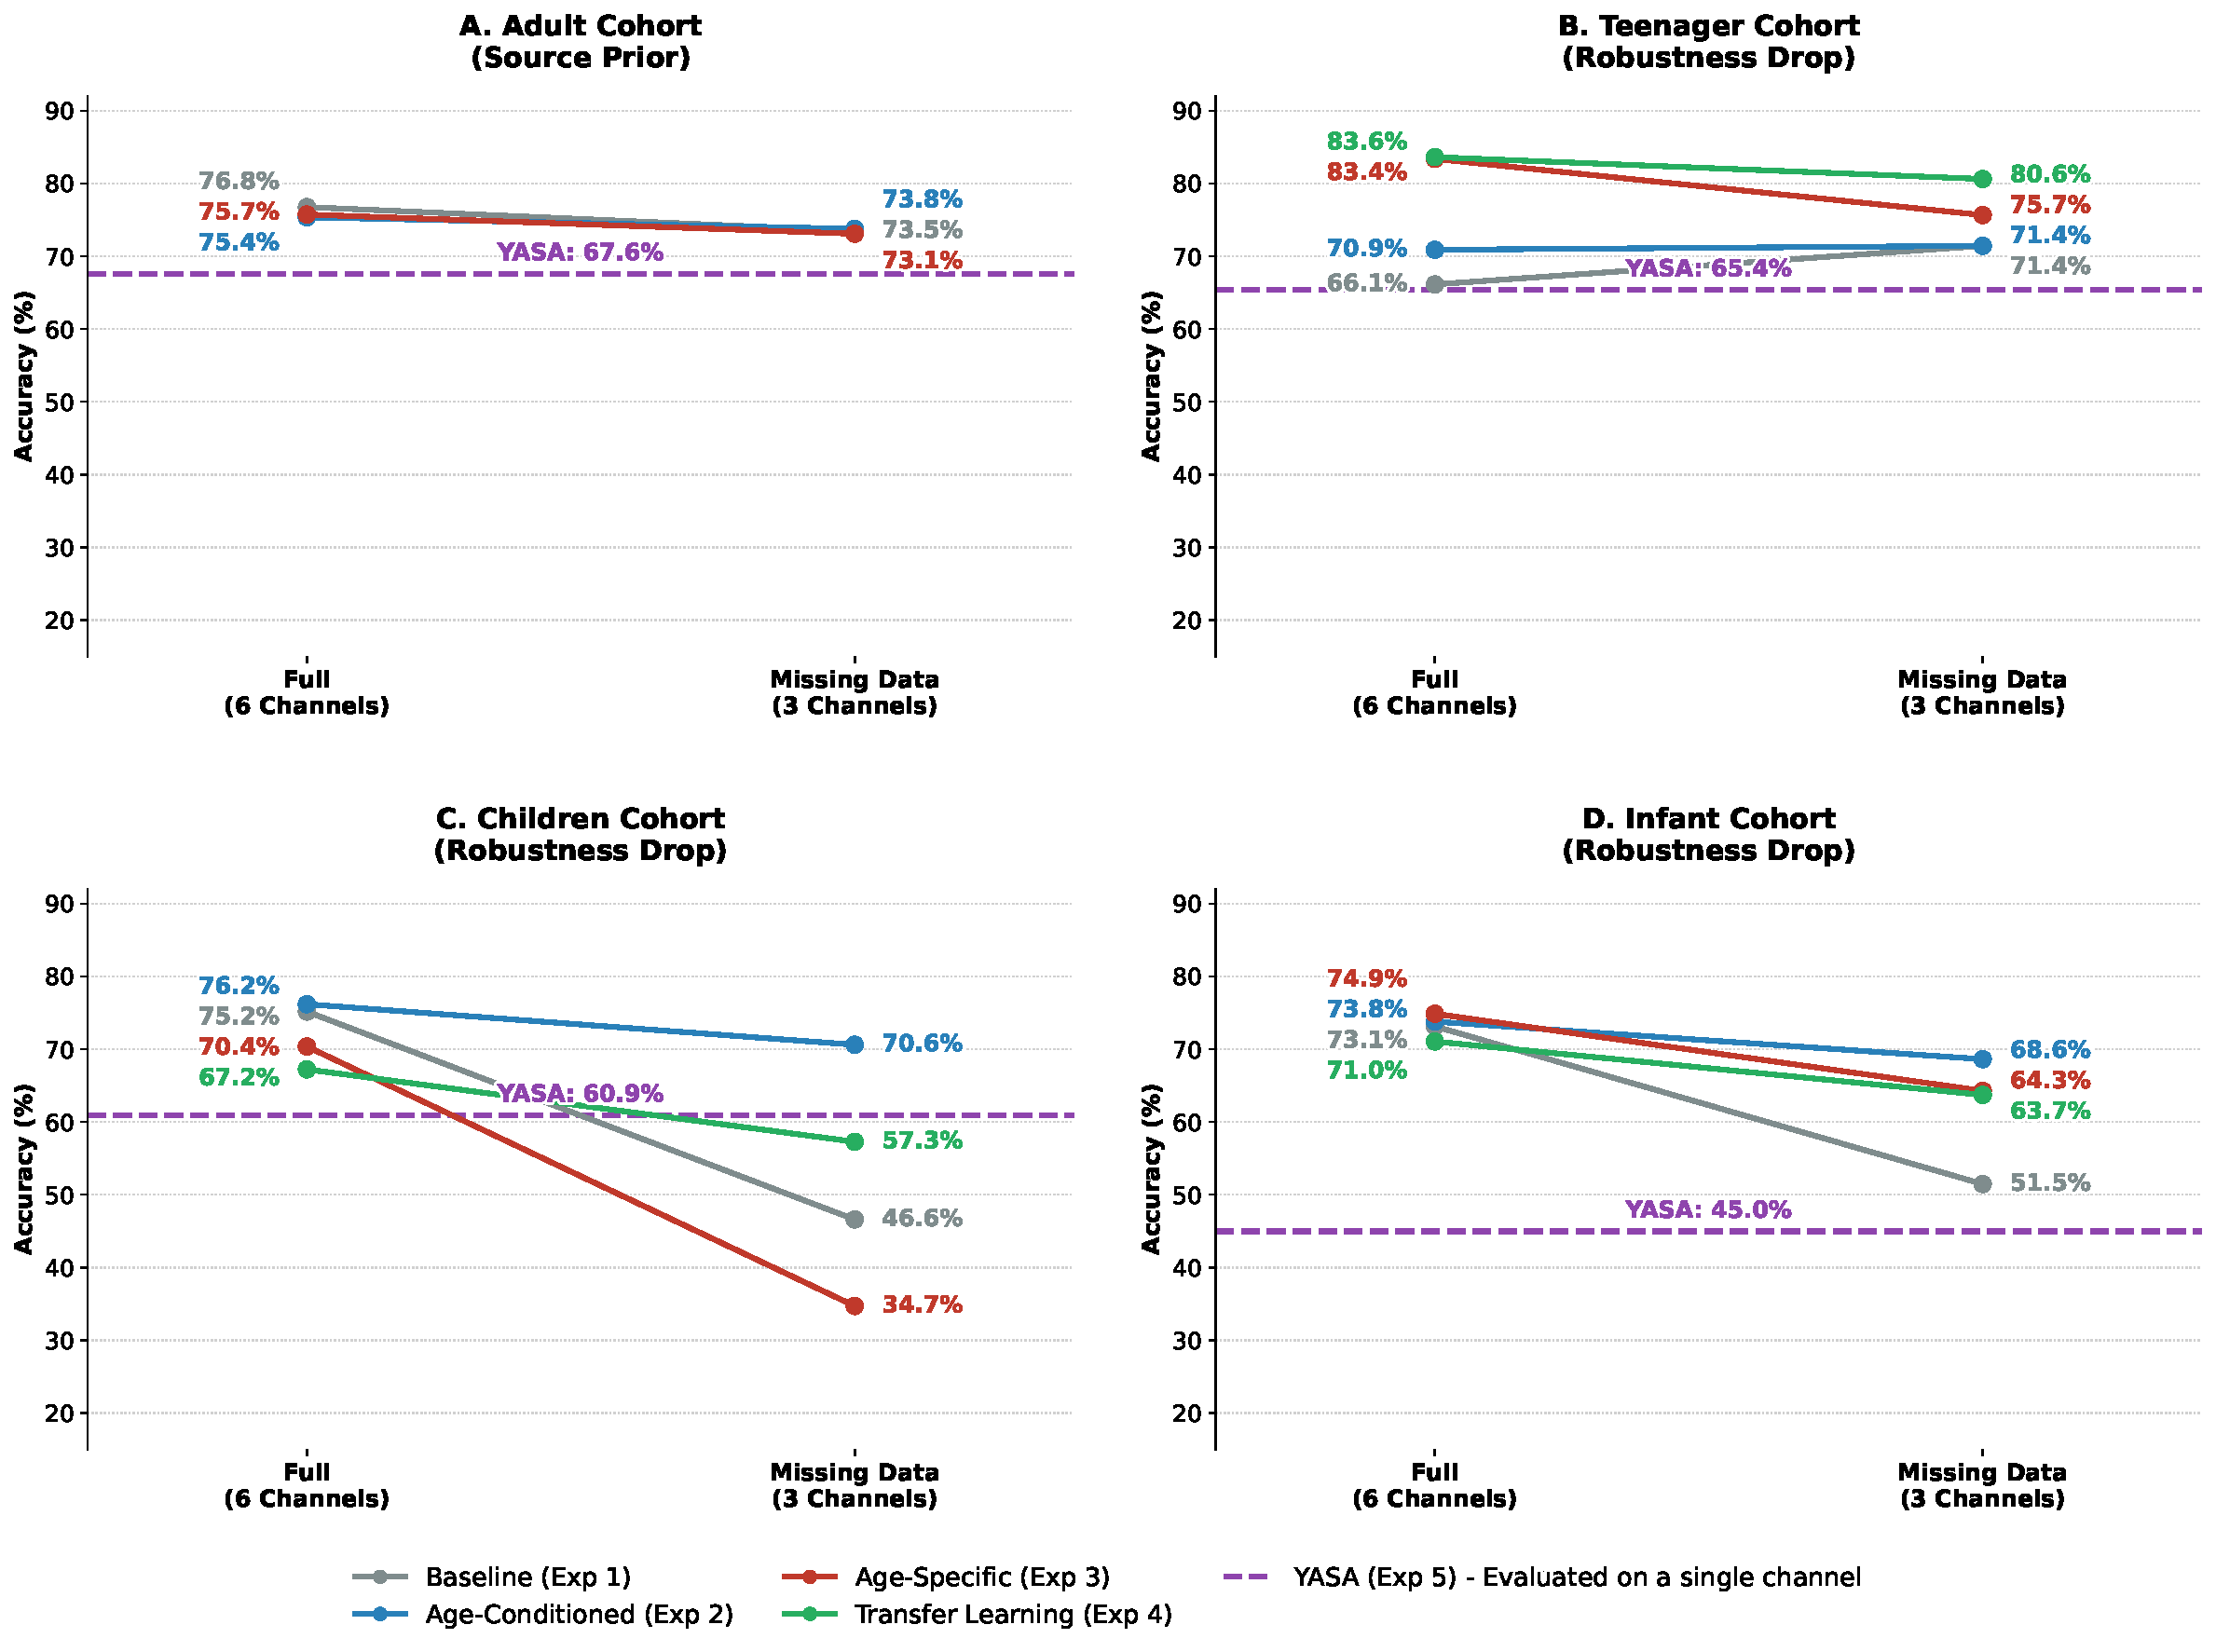
\includegraphics[height=0.98\textheight, keepaspectratio]{experiments_slope_chart.pdf}
    \vspace{0.5cm}
    \caption{\textbf{Cross-Experiment Comparison and Sensor Loss Robustness.}  This slope chart visualizes accuracy degradation when models encounter missing channels at inference. It shows how demographic conditioning and transfer learning buffer younger cohorts against sensor loss.}
    \label{fig:overall_comparison}
\end{figure}
\end{landscape}

\section{Age-Routed Sleep Staging Framework}
\label{sec:routing_framework}

The preceding evaluations (Experiments 1 through 4) demonstrate that no single architectural setup achieves optimal performance
and robustness across all developmental stages. While adult and adolescent recordings benefit from broad spatial configurations
and transfer learning, dedicated age-specific networks best capture infant sleep, and the data-starved children
cohort requires the regularization that demographic conditioning provides.

We used these findings to develop a simple, age-routed
inference framework. Instead of relying on a specific architecture, this framework dynamically selects and deploys
the optimally performing model configuration we found in previous experiments based on the patient's biological age 
at the time of the recording. 

When we provide a new recording, the pipeline extracts the patient's age and routes the sequence of 30-second
EEG spectrograms to one of four specialized, pre-trained networks:
\begin{itemize}
    \item \textbf{adults (Age $\geq$ 18 years):} we process the sequence with the standard generalist baseline model (Experiment 1), which benefits from the massive dataset,
    \item \textbf{teenagers (12 to 18 years):} we route it to the fine-tuned transfer learning model (Experiment 4), which successfully adapts adult spatial priors to adolescent waveforms,
    \item \textbf{children (2 to 12 years):} we handle it with the age-conditioned model (Experiment 2), which requires an explicit demographic embedding tensor,
    \item \textbf{infants ($<$ 2 years):} we evaluate it using the natively trained age-specific network (Experiment 3), which best captures the highly distinct EEG patterns unique to early pediatric development.
\end{itemize}
If the patient's age is missing, the router falls back to the baseline model, which was trained on all age groups.

Each demographic cohort exposes both the full 6-channel variant and the natively trained 3-channel variant evaluated earlier in this chapter. 
If a recording contains more than 3 channels, the framework selects the 6-channel variant. If it contains 3 or fewer channels, it automatically
routes the input to the natively trained 3-channel variant. Should a recording still differ from the selected variant's expected channel count
(for example, 1 or 2 channels routed to a 3-channel model), the pipeline zero-pads the missing dimensions.

Prior to inference, each recording is standardized using the exact training-set mean and standard deviation associated with the
selected cohort and channel variant. When ground-truth stage annotations are available the framework automatically computes per-recording and
aggregate evaluation metrics (accuracy, Cohen's Kappa, macro F1 and confusion matrices). By harmonizing these architectural and spatial-resolution
strategies into a single programmatic interface, the framework maximizes predictive accuracy and clinical robustness across all studied developmental stages of this thesis.


\chapter{Conclusion}
Sleep staging is a complex clinical task that has traditionally been performed by 
human experts who meticulously analyze continuous physiological recordings.
Recently, researchers have increasingly utilized deep learning models to automate and scale
this process. In this thesis, we developed a deep neural network based on the Transformer
architecture to classify sleep stages from raw EEG signals. We demonstrated the inherent limitations
of a generalist baseline model that processes data without demographic context, and we
subsequently introduced and evaluated three distinct methodologies for incorporating patient age
to improve generalization and robustness.

Our baseline evaluations revealed that while the unconditioned model performed well on the largest adult dataset,
it struggled to generalize across other developmental stages, exposing two critical vulnerabilities: an over-reliance
on information shared across channels and demographic bias. For underrepresented cohorts, such as children and infants,
the full 6-channel model achieved decent accuracy by exploiting dependencies between channels that did not generalize well.
This became evident when evaluating the model using only 3 channels, which caused predictive accuracy for
these younger cohorts to collapse catastrophically.

Conversely, the model exhibited a different yet equally severe limitation when processing teenage data. When we evaluated the model on all 6 channels, accuracy for teenagers was the lowest among all cohorts; however, accuracy substantially improved when we reduced the spatial dimensionality to 3 channels. 

We argue this anomaly stems from the interaction between extreme dataset imbalance and adolescent neurodevelopment. Because teenagers share fundamental temporal sleep dynamics with adults, the network attempted to map teenage recordings into the dominant adult feature space. However, due to ongoing adolescent brain maturation, teenage EEG exhibits distinct amplitudes and spatial distributions compared to adult sleep. When evaluating across all 6 channels, these spatial differences conflicted with the network's adult-biased spatial filters, acting as noise. 
We hypothesize that reducing the input dimensionality to 3 channels effectively provided architectural regularization: by removing the extra spatial channels, we prevented the network from enforcing rigid adult spatial rules, allowing it to leverage the shared temporal sleep features that generalize across both demographics.

To address these demographic disparities, our first proposed solution 
incorporated the patient's age cohort as an explicit demographic prior 
via an additional embedding layer. By offloading the task of age deduction,
the network was able to learn cohort-specific representations without having
to implicitly extract developmental stages from the raw EEG data. 
While this balancing effect resulted in a marginal decrease in adult accuracy,
performance on the underrepresented and morphologically distinct cohorts improved significantly.
Most crucially, this demographic conditioning served as a powerful 
regularizer against spatial brittleness. When evaluating on only 3 channels,
we successfully mitigated the catastrophic performance collapse we previously observed in the children cohort,
maintaining a significantly higher stability.

Interestingly, we observed an anomaly when we natively trained and evaluated the age-conditioned model
on only 3 channels: accuracy for 
the teenage cohort actually decreased (77.38\%) compared to the 
unconditioned 3-channel baseline (81.28\%). We speculate that this 
drop is a consequence of representational partitioning. In the unconditioned 
3-channel baseline, the absence of age group information allowed teenagers 
to seamlessly leverage the massive volume of shared features learned from the 
adult majority. By explicitly providing an age embedding, the conditioned model 
artificially segregated the teenage representations from the adults. 
Because their core temporal waveforms are highly similar, this 
explicit separation prevented the teenage cohort from fully capitalizing
on the shared adult temporal priors, demonstrating that demographic conditioning 
can occasionally hinder transferability when the underlying domain features are 
already strongly aligned.

To further investigate the impact of demographic variance, our second approach
completely partitioned the dataset to train independent, age-specific models.
Rather than processing all cohorts through shared temporal and spatial weights,
this isolation allowed each network to optimize its feature extraction exclusively
for its target demographic. However, this approach exposed a critical vulnerability
regarding dataset volume. The specialized model for the children cohort, which
possessed the fewest training samples, yielded the poorest overall native
performance (70.37\%). Furthermore, when we subjected this model to the 3-channel missing data
simulation, its accuracy catastrophically plummeted to 34.69\%. This
confirms that in the absence of sufficient training data, the full 6-channel
spatial resolution leads to overparameterization.

Conversely, partitioning the dataset yielded mixed but highly illuminating 
results for the larger cohorts. The isolated adult model actually underperformed 
the generalist baseline (75.74\% vs. 76.76\%), indicating that the baseline network
benefited from the regularization and diversity provided by the aggregate dataset
(which included over 310,000 total samples across all ages). However, the
age-specific approach proved exceptionally beneficial for the teenage cohort,
achieving an impressive 83.38\% accuracy on the full spatial resolution. We attribute
this surge in performance to the network's ability to calibrate its spatial filters
directly to adolescent-specific distributions. Unlike the children
cohort, the teenage dataset was sufficiently large to avoid severe overfitting.
Freed from the dominant adult spatial biases that constrained the baseline and
conditioned models, the isolated teenage network could fully leverage all 6
channels to learn optimized, robust representations unique to adolescent sleep
architecture.

To address the data scarcity we observed in the younger demographics, our third
proposed solution utilized transfer learning. By utilizing the partitioned adult
networks as base models, we aimed to leverage foundational sleep features learned
from the massive adult majority and fine-tune them on the smaller,
underrepresented cohorts. This approach, however, yielded a complex trade-off
between absolute peak performance and diagnostic robustness. When we trained and
evaluated children and infant models on the full 6-channel resolution, they slightly
underperformed their from-scratch, age-specific counterparts. We attribute this
to weight anchoring and negative transfer; we had so deeply optimized the pre-trained spatial filters
for adult neurophysiology that the network struggled to fully
adapt them to the unique spatial topographies of children and infants during fine-tuning.

Despite this slight drop in peak accuracy, transfer learning demonstrated
profound clinical value in mitigating spatial brittleness for data-starved
cohorts. When we subjected the fine-tuned children's model to the simulated loss
of 3 channels, it maintained an accuracy of 57.27\%—a massive 23 percentage point 
improvement over the catastrophic 34.69\% crash we observed in the isolated model. 
By grounding the network in generalized adult priors, the fine-tuning process
successfully prevented the data-scarce children's model from memorizing
brittle spatial shortcuts. Finally, this experiment reinforced our previous findings
regarding architectural regularization: for the infant cohort,
fine-tuning a natively 3-channel model actually outperformed fine-tuning the
6-channel model. By restricting the spatial dimensions during transfer learning,
we successfully stripped away the rigid, adult-specific spatial biases, allowing
the network to cleanly transfer highly generalizable temporal sleep waveforms
across different age stages.

Finally, to contextualize our contributions against established clinical software,
we evaluated our architectures against YASA (Yet Another Spindle Algorithm),
a popular off-the-shelf sleep staging tool. Even under an optimistic evaluation
protocol that granted YASA the optimal demographic assumptions, the model achieved
an average accuracy of 67.60\% for adults, 65.39\% for teenagers, 60.94\% for children,
and a mere 44.96\% for infants. Across every demographic cohort, our proposed
Transformer architectures substantially outperformed this established baseline.
Our unconditioned model achieved higher accuracy on adults (76.76\% vs. 67.60\%),
while our demographic-aware approaches dramatically outpaced YASA on younger
cohorts—most notably for teenagers (reaching 83.38\% vs. 65.39\%) and children
(reaching 76.18\% vs. 60.94\%).

We observed the most profound gap in the infant cohort, where our age-conditioned
and age-specific models outperformed YASA by nearly 30 percentage points (73.79\%
and 74.87\%, respectively, vs. 44.96\%). This dramatic performance collapse in the
established model underscores a critical limitation of traditional off-the-shelf
tools: because they rely on single-channel rules and feature extractors trained
predominantly on adult populations, they fail to generalize to the
pediatric populations. Ultimately, this comparison
validates the core motivation of this thesis, proving that off-the-shelf software is
ill-equipped for non-adult sleep staging and demonstrating the necessity of age-aware
deep learning models.

Through these experiments, this thesis has demonstrated the critical importance
of explicitly accounting for demographic variance in deep learning models
for sleep staging. Furthermore, our findings highlight a significant
methodological risk: relying solely on standard test-set accuracy can yield
misleading conclusions regarding model competence. As we demonstrated, seemingly
minor data changes such as the simulated loss of a few clinical sensors 
can expose severe spatial brittleness and trigger catastrophic 
performance degradation. Consequently, when developing models intended for 
clinical generalization, it is important to subject them to rigorous 
stress-testing across multiple real-world failure scenarios.

While this research focused exclusively on patient age, it is highly probable
that similar representational biases exist across other demographic variables,
such as neurological health conditions or underlying sleep disorders,
which also fundamentally alter EEG morphology. A natural limitation of
this study is the absence of prospective validation in a live clinical
environment. Future work should prioritize deploying these networks alongside
human sleep experts to directly compare the models' generalized representations
against established clinical workflows. Ultimately, however, this thesis
establishes the profound potential of Transformer architectures for
automated sleep staging, proving their high clinical utility when datasets
and training methodologies are carefully designed to balance both accuracy and robustness.
%----------------------------------------------------------------
% SLO: bibliografija
% ENG: bibliography
%----------------------------------------------------------------
\bibliographystyle{elsarticle-num}
%----------------------------------------------------------------
% SLO: odkomentiraj za uporabo zunanje datoteke .bib (ne pozabi je potem prevesti!)
% ENG: uncomment to use .bib file (don't forget to compile it!)
%----------------------------------------------------------------
\bibliography{bibliography}

%----------------------------------------------------------------
% SLO: zakomentiraj spodnji del, če uporabljaš zunanjo .bib datoteko
% ENG: comment the part below if using the .bib file
%----------------------------------------------------------------

% \begin{thebibliography}{99}
% \bibitem{Fortnow} L.\ Fortnow, ``Viewpoint: Time for computer science to grow up'',
% {\it Communications of the ACM}, št.\ 52, zv.\ 8, str.\ 33--35, 2009.
% \bibitem{Knuth} D.\ E.\ Knuth, P. Bendix. ``Simple word problems in universal algebras'', v zborniku: Computational Problems in Abstract Algebra (ur. J. Leech), 1970, str. 263--297.
% \bibitem{Lamport} L.\ Lamport. {\it LaTEX: A Document Preparation System}. Addison-Wesley, 1986.
% \bibitem{ubi} O.\ Patashnik (1998) \BibTeX{}ing.
% Dostopno na: \url{http://ftp.univie.ac.at/packages/tex/biblio/bibtex/contrib/doc/btxdoc.pdf}
% \bibitem{licence} licence-cc.pdf. Dostopno na: \url{https://ucilnica.fri.uni-lj.si/course/view.php?id=274}
% \end{thebibliography}

\end{document}
